\documentclass[11pt,a4paper,twoside]{tesis}  % puede agregarse `twoside` como opción si se necesita "formato libro"

\usepackage{graphicx}
\usepackage[utf8]{inputenc}
\usepackage[spanish]{babel}
\usepackage[left=3cm,right=3cm,bottom=3.5cm,top=3.5cm]{geometry}

\usepackage{biblatex}
\usepackage{csquotes}  % https://tex.stackexchange.com/a/229653
\addbibresource{refs/eye_tracking.bib}
\addbibresource{refs/neuro_tools.bib}
\addbibresource{refs/antisaccades_task.bib}
\addbibresource{refs/saccades.bib}
\addbibresource{refs/other_areas.bib}

% algunas constantes para asegurarme de que quede todo parejo
\usepackage{xspace}  % para garantizar un espacio dsp de los newcommand
                     % https://tex.stackexchange.com/a/17731
\newcommand{\eyetracking}{\textit{eye tracking}\xspace}
\newcommand{\eyetrackingweb}{\eyetracking web\xspace}
\newcommand{\eyetracker}{\textit{eye tracker}\xspace}
\newcommand{\eyetrackers}{\textit{eye trackers}\xspace}
\newcommand{\js}{\texttt{JavaScript}\xspace}
\newcommand{\jspsych}{\texttt{JSPsych}\xspace}
\newcommand{\pupilext}{\texttt{PupilEXT}\xspace}
\newcommand{\psychophysics}{\texttt{PsychoPhysics}\xspace}
\newcommand{\turkergaze}{\texttt{TurkerGaze}\xspace}
\newcommand{\webgazer}{\texttt{WebGazer}\xspace}
\newcommand{\pace}{\texttt{PACE}\xspace}
\newcommand{\rastoc}{\texttt{rastoc}\xspace}

\usepackage{svg}  % https://tex.stackexchange.com/a/445182/273585

\usepackage{hyperref}  % clickable links

\usepackage{enumitem}         % reduce space between itemize's items 
\setlist[itemize]{noitemsep}  % https://tex.stackexchange.com/a/457737/273585

\usepackage[T1]{fontenc}  % https://tex.stackexchange.com/a/1775/273585

\begin{document}

\def\autor{Francisco Figari}
\def\tituloTesis{Aplicaciones de eye tracking online en diagnóstico de
condiciones neuropsicológicas}
\def\runtitulo{Aplicaciones de eye tracking online en diagnóstico de
condiciones neuropsicológicas}
%\def\runtitle{Star Wars: Rebellion and Empire}
\def\director{Juan Kamienkowski}
\def\codirector{Gustavo Juantorena}
\def\lugar{Buenos Aires, 2022}
\input{caratula}

%%%% ABSTRACTS, AGRADECIMIENTOS Y DEDICATORIA
\frontmatter
\pagestyle{empty}
\input{abs_esp.tex}

%\cleardoublepage
%\input{abs_en.tex} % OPCIONAL: comentar si no se quiere

%\cleardoublepage
%\input{agradecimientos.tex} % OPCIONAL: comentar si no se quiere

%\cleardoublepage
%\vspace*{\fill}

\hfill\textit{A mis directores, al LIAA, al DC}

\hfill\textit{A ma, pa, Mati, Juan y Sofi}

\hfill\textit{A quienes con su brillo iluminan el camino}
  % OPCIONAL: comentar si no se quiere

\cleardoublepage
\tableofcontents

\mainmatter
\pagestyle{headings}

\documentclass[aspectratio=169]{beamer}

\usepackage{subcaption}
\usepackage{emoji}

\title{Evaluación y desarrollo de \textit{eye tracking} remoto en navegadores
\textit{web}}
\author{Francisco Figari, Juan Kamienkowski, Gustavo Juantorena, Bruno Bianchi}
\date{Buenos Aires, 2022}
\titlegraphic{
\includegraphics[width=8em]{img/logo-fcen.png}}

\setbeamertemplate{navigation symbols}{}

% TODO: Hacer que esto sea opcional
\setbeamertemplate{frametitle}{
  \insertsectionhead\par
  \vspace*{0.2mm}
  \insertsubsectionhead\par
  \vspace*{0.2mm}
  \insertframetitle
}

\begin{document}

\frame{\titlepage}

\section{Implementación}

\begin{frame}{\texttt{WebGazer} como punto de partida}

  \begin{columns}
    \begin{column}{.5\textwidth}
      \begin{itemize}
        \item[\emoji{thumbs-up}] Extracción de frames a través de la API del
          navegador
        \item[\emoji{thumbs-up}] Modelos de localización de los ojos y de
          estimación de la mirada
        \item[\emoji{thumbs-down}] Calibración inadecuada
        \item[\emoji{thumbs-down}] Ausencia de notificación de descalibraciones
        \item[\emoji{party-popper}] Corrregida falla de \texttt{WebGazer} que
          causaba \textit{crashes} del navegador en ciertas notebooks
      \end{itemize}
    \end{column}

    \begin{column}{.5\textwidth}
      \begin{figure}
        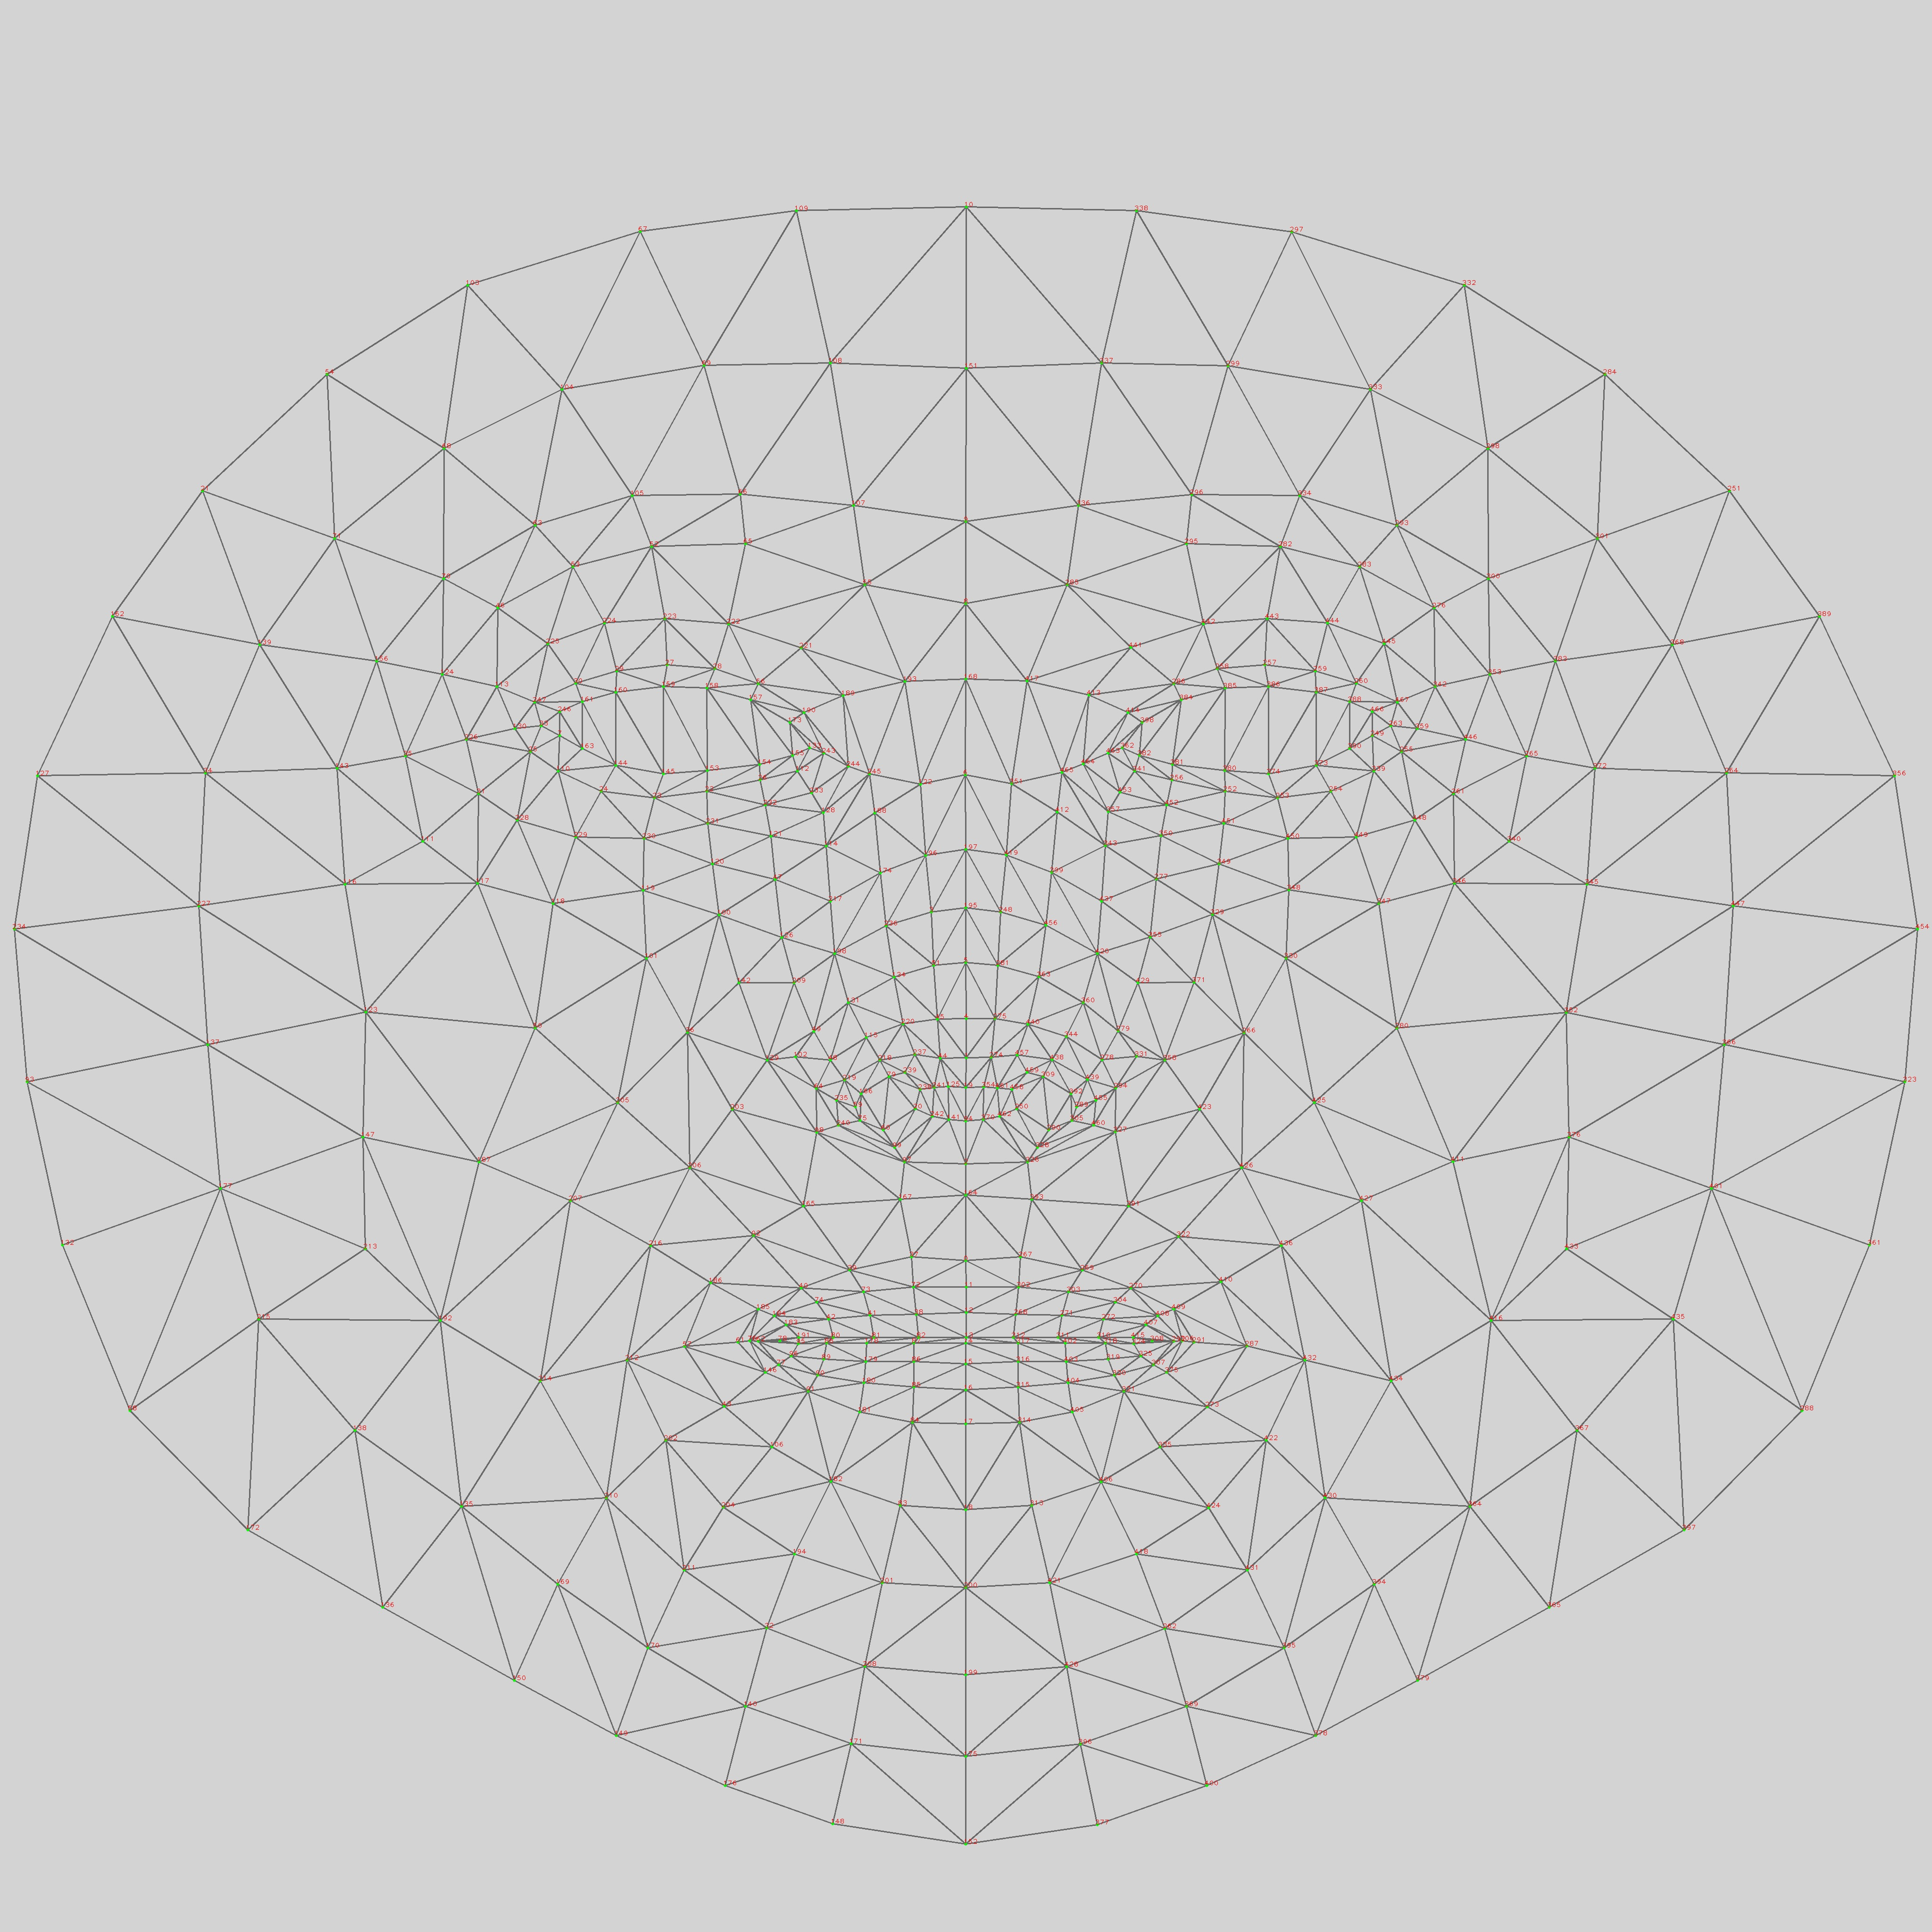
\includegraphics[width=0.75\linewidth]{img/facemesh-kepyoints.jpg}
        \caption{\textit{Output} del modelo de \textit{facemesh} utilizado por
        \texttt{WebGazer} para la localización de los ojos}
      \end{figure}
    \end{column}
  \end{columns}

\end{frame}

\begin{frame}{Calibración y validación}
  \begin{itemize}
    \item Nuestro caso de uso no garantiza interacciones

    \item Se muestran una serie de puntos, para cada uno de los cuales el
      usuario tendrá que fijar la mirada y presionar la barra de espacio
    
    \item Validación post calibración implementada de similar manera

    \item[\emoji{party-popper}] \texttt{WebGazer} adaptado para evitar cómputos
      ya no necesarios
  \end{itemize}
\end{frame}

\begin{frame}{Notificación de descalibración}

  \begin{columns}
    \begin{column}{.5\textwidth}
      \begin{itemize}
        \item Basada en detectar movimiento
        \item Instanciada luego de cada calibración
        \item Verificación realizada para cada \textit{frame}
        \item \emoji{party-popper} \texttt{WebGazer} adaptado para exponer los
          recuadros calculados en cada \textit{frame} por la rutina de
          localización de ojos
      \end{itemize}
    \end{column}

    \begin{column}{.5\textwidth}
      \begin{figure}
        \centering
        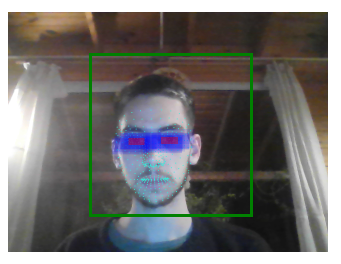
\includegraphics[width=\textwidth]{img/eyetracker-playground-screenshot.png}
        \caption{Detección de movimiento en funcionamiento}
      \end{figure}
    \end{column}
  \end{columns}

\end{frame}

\section{Experimentación}

\begin{frame}{Caso de estudio: tarea de antisacadas}

  \begin{columns}
    \begin{column}{.5\textwidth}
      \begin{itemize}
        \item Clínicamente relevante
        \item Resultados esperados ya establecidos
        \item Tarea simple para validar movimientos oculares
      \end{itemize}
    \end{column}
    \begin{column}{.5\textwidth}
      \begin{figure}
        \centering
        \includegraphics[width=\linewidth]{img/antisaccades-protocol.png}
        \caption{Protocolo de las tareas}
      \end{figure}
    \end{column}
  \end{columns}

\end{frame}

\begin{frame}{Primera instancia}
  \begin{itemize}
    \item Limitados a 10 minutos debido a una falla de \texttt{WebGazer}
    \item Únicamente ensayos de antisacada
    \item Recalibración luego de cada notificación de descalibración
    \item Sin validación post calibración
  \end{itemize}
\end{frame}

\begin{frame}{Segunda instancia}
  \begin{itemize}
    \item Duración superior a 20 minutos
    \item Ensayos de prosacadas y de antisacadas
    \item Recalibración cada 10 ensayos y sólo si se detectó una
      descalibración
    \item Con validación post calibración
  \end{itemize}
\end{frame}

\begin{frame}{Implementación y distribución}

  \begin{columns}
    \begin{column}{0.4\textwidth}
      \begin{figure}
        \centering
        
\includegraphics[width=\textwidth]{img/jspsych-logo.jpg}
      \end{figure}
    \end{column}
    \begin{column}{0.6\textwidth}
      \begin{figure}
        \centering
        
\includegraphics[width=0.8\textwidth]{img/cognition-run-logo.png}
        
\includegraphics[width=\textwidth]{img/neuropruebas-logo.jpg}
      \end{figure}
    \end{column}
  \end{columns}
\end{frame}


\section{Resultados}

\begin{frame}{Ejemplo de \textit{output} del sistema}
  \begin{figure}
    \centering
    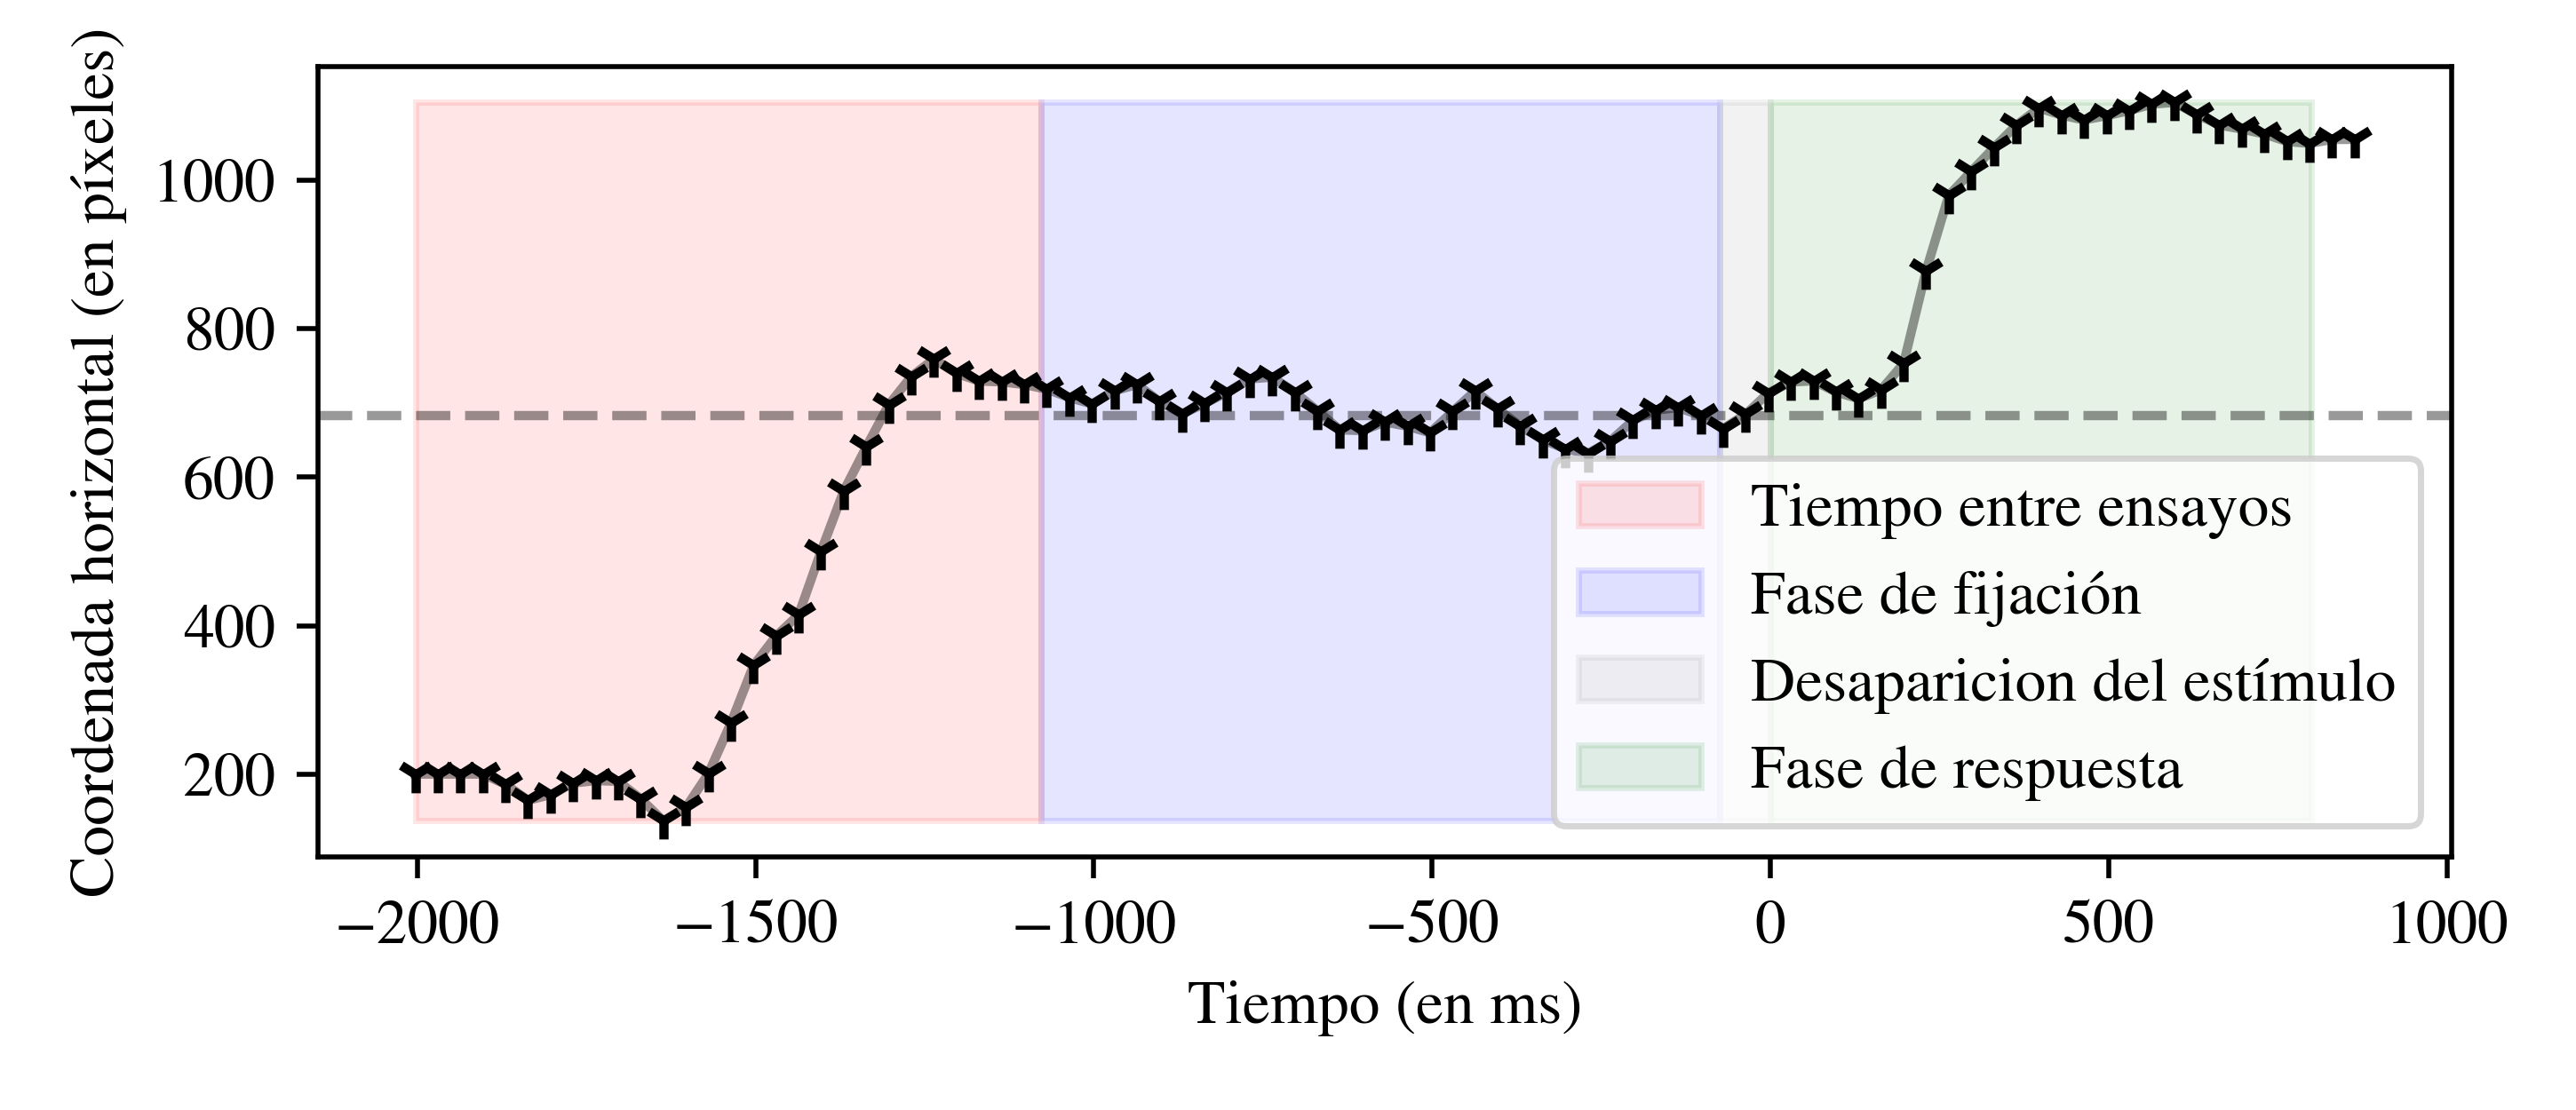
\includegraphics[width=\linewidth]{plots/output-example.png}
  \end{figure}
\end{frame}

\begin{frame}{Frecuencias de muestreo}
  \begin{figure}
    \centering
    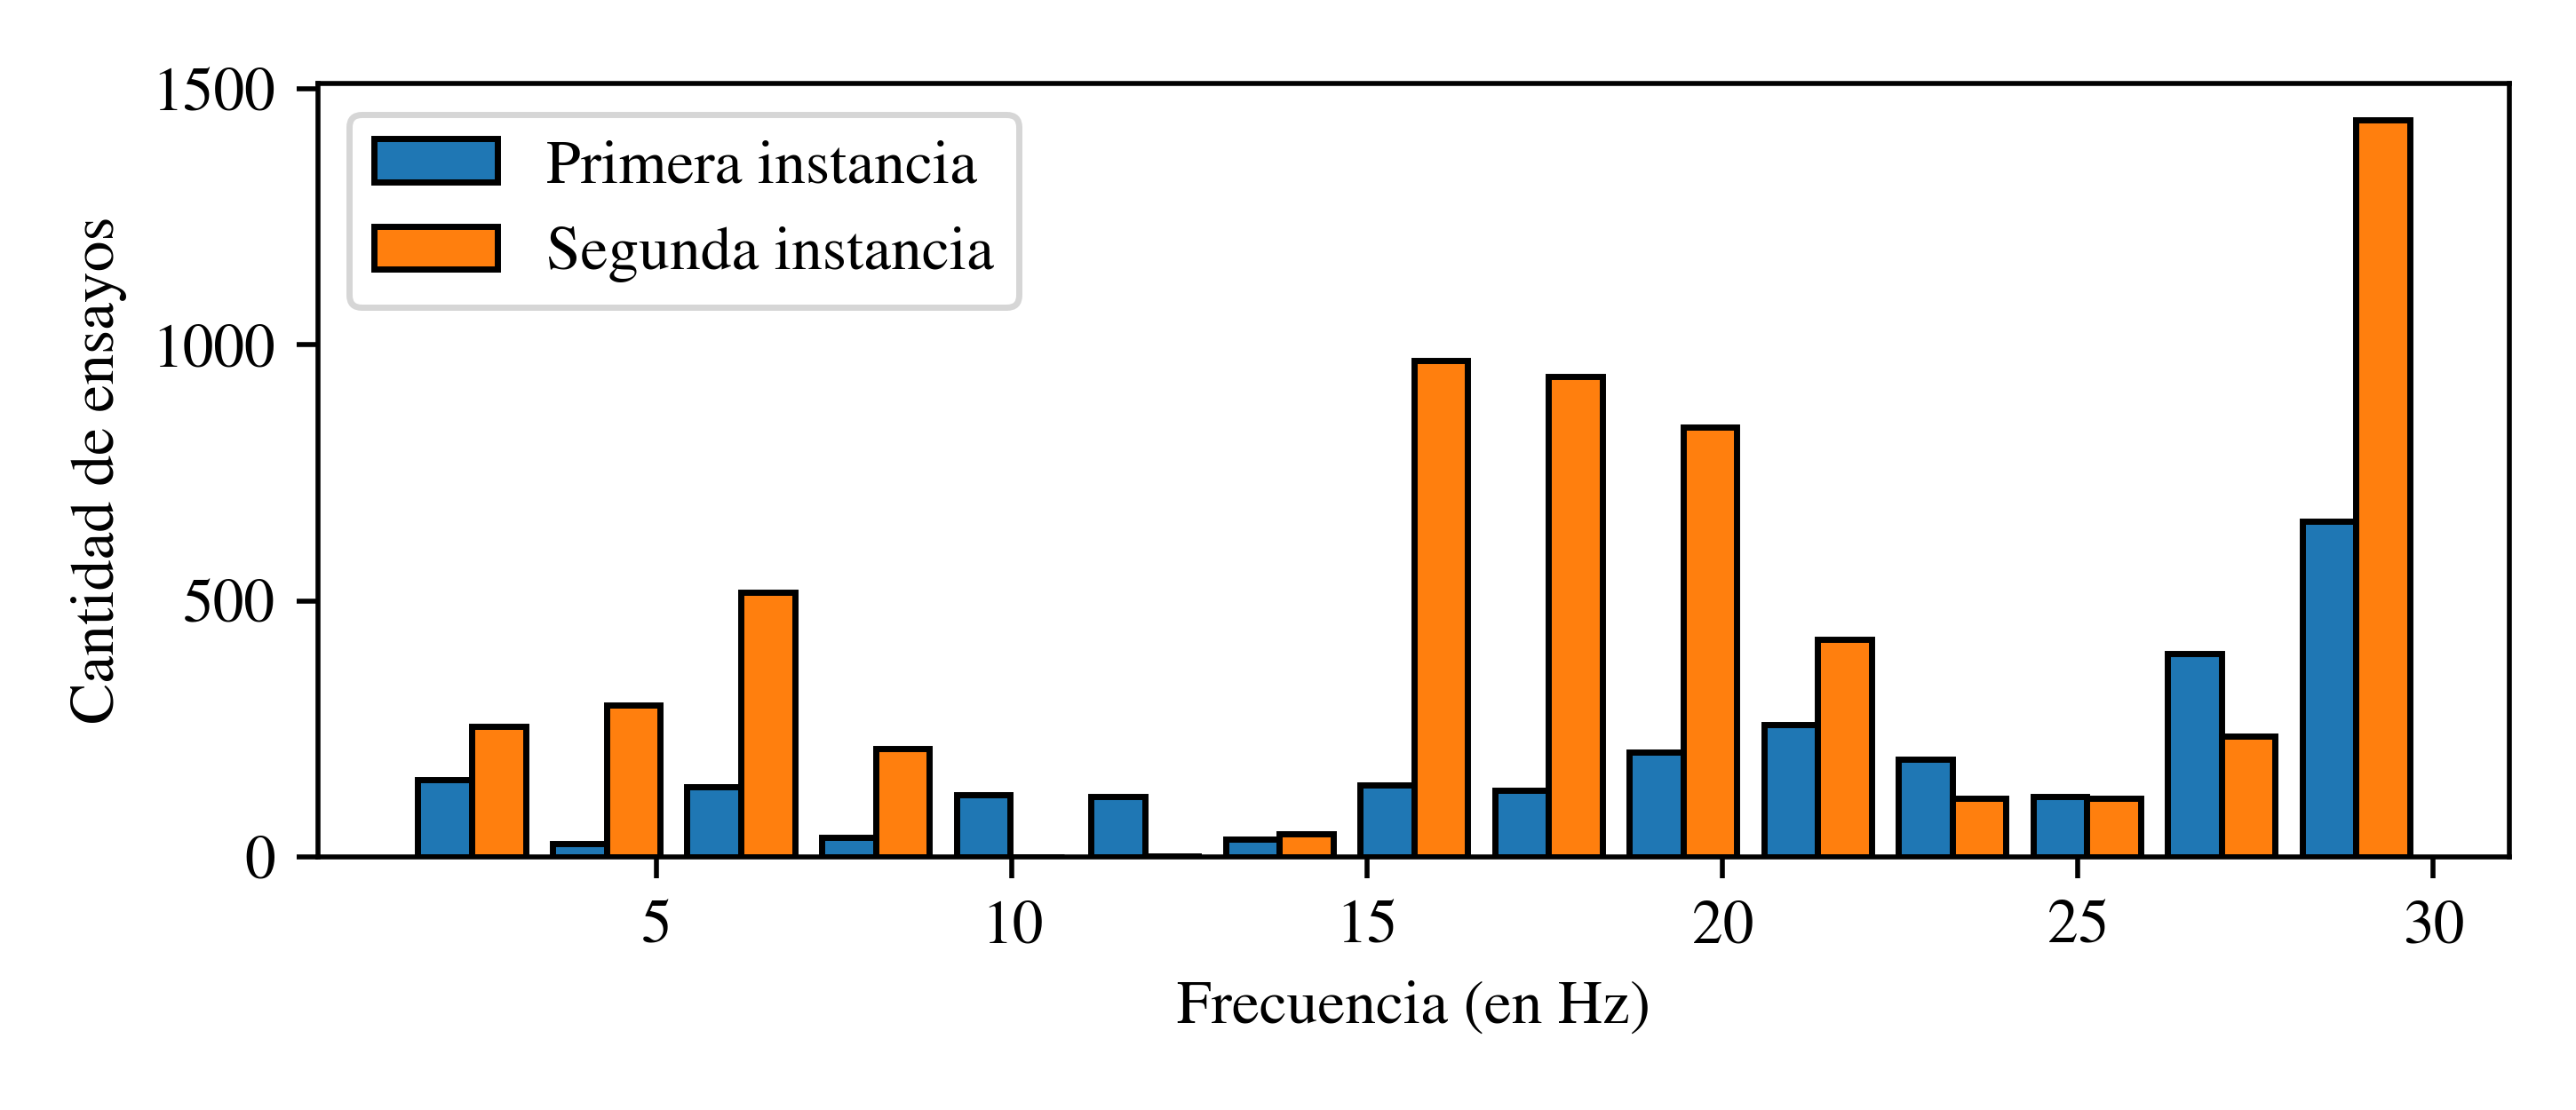
\includegraphics[width=\linewidth]{plots/sampling-frequencies-distribution.png}
  \end{figure}
\end{frame}

\begin{frame}{Anchos de pantalla}
  \begin{figure}
    \centering
    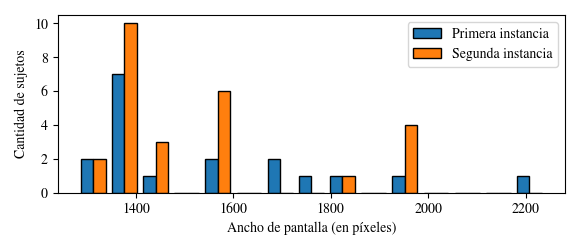
\includegraphics[width=\linewidth]{plots/screens-widths-distribution.png}
  \end{figure}
\end{frame}

\begin{frame}{Estimaciones desviadas}
  \begin{figure}
    \centering
    \includegraphics[width=\linewidth]{plots/skewed-estimations-examples.png}
    \caption{Las estimaciones de algunos sujetos están desviadas de los valores reales}
  \end{figure}
\end{frame}

\begin{frame}{Limpieza y normalización}
  \begin{columns}
    \begin{column}{0.4\textwidth}
      \begin{itemize}
        \item Ensayos descartados: \begin{itemize}
          \item frecuencia menor a 15 Hz
          \item a mano
          \item si el sujeto se distrajo de la tarea
        \end{itemize}
        \item Frecuencia de muestreo: \textit{Upsampling} a 30 Hz usando
          interpolación lineal
      \end{itemize}
    \end{column}
    \begin{column}{0.6\textwidth}
      \begin{figure}
        \centering
        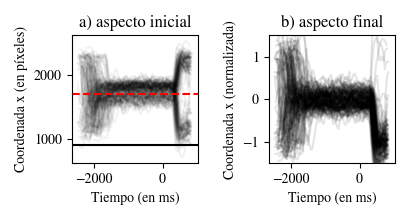
\includegraphics[width=\linewidth]{plots/normalization-example.png}
        \caption{Normalizado y espejado}
      \end{figure}
    \end{column}
  \end{columns}
\end{frame}

\begin{frame}{Detección de sacadas}
  \begin{columns}
    \begin{column}{0.5\textwidth}
      \begin{figure}
        \centering
        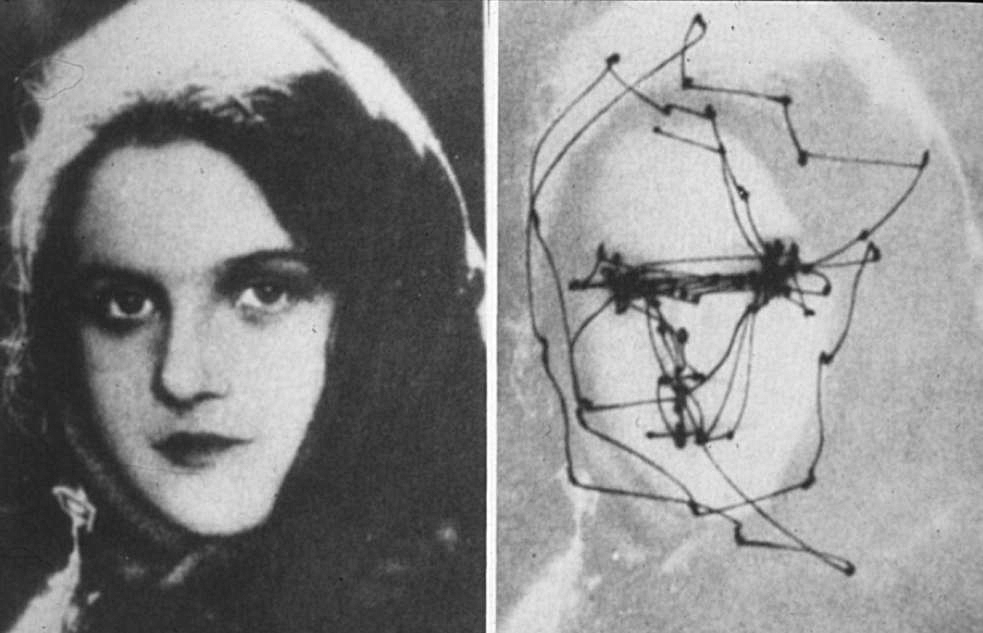
\includegraphics[width=\linewidth]{img/saccades-example.jpg}
        \caption{Los movimientos oculares muestran qué elementos de una imagen
        capturan la atención}
      \end{figure}
    \end{column}
    \begin{column}{0.5\textwidth}
      \begin{figure}
        \centering
        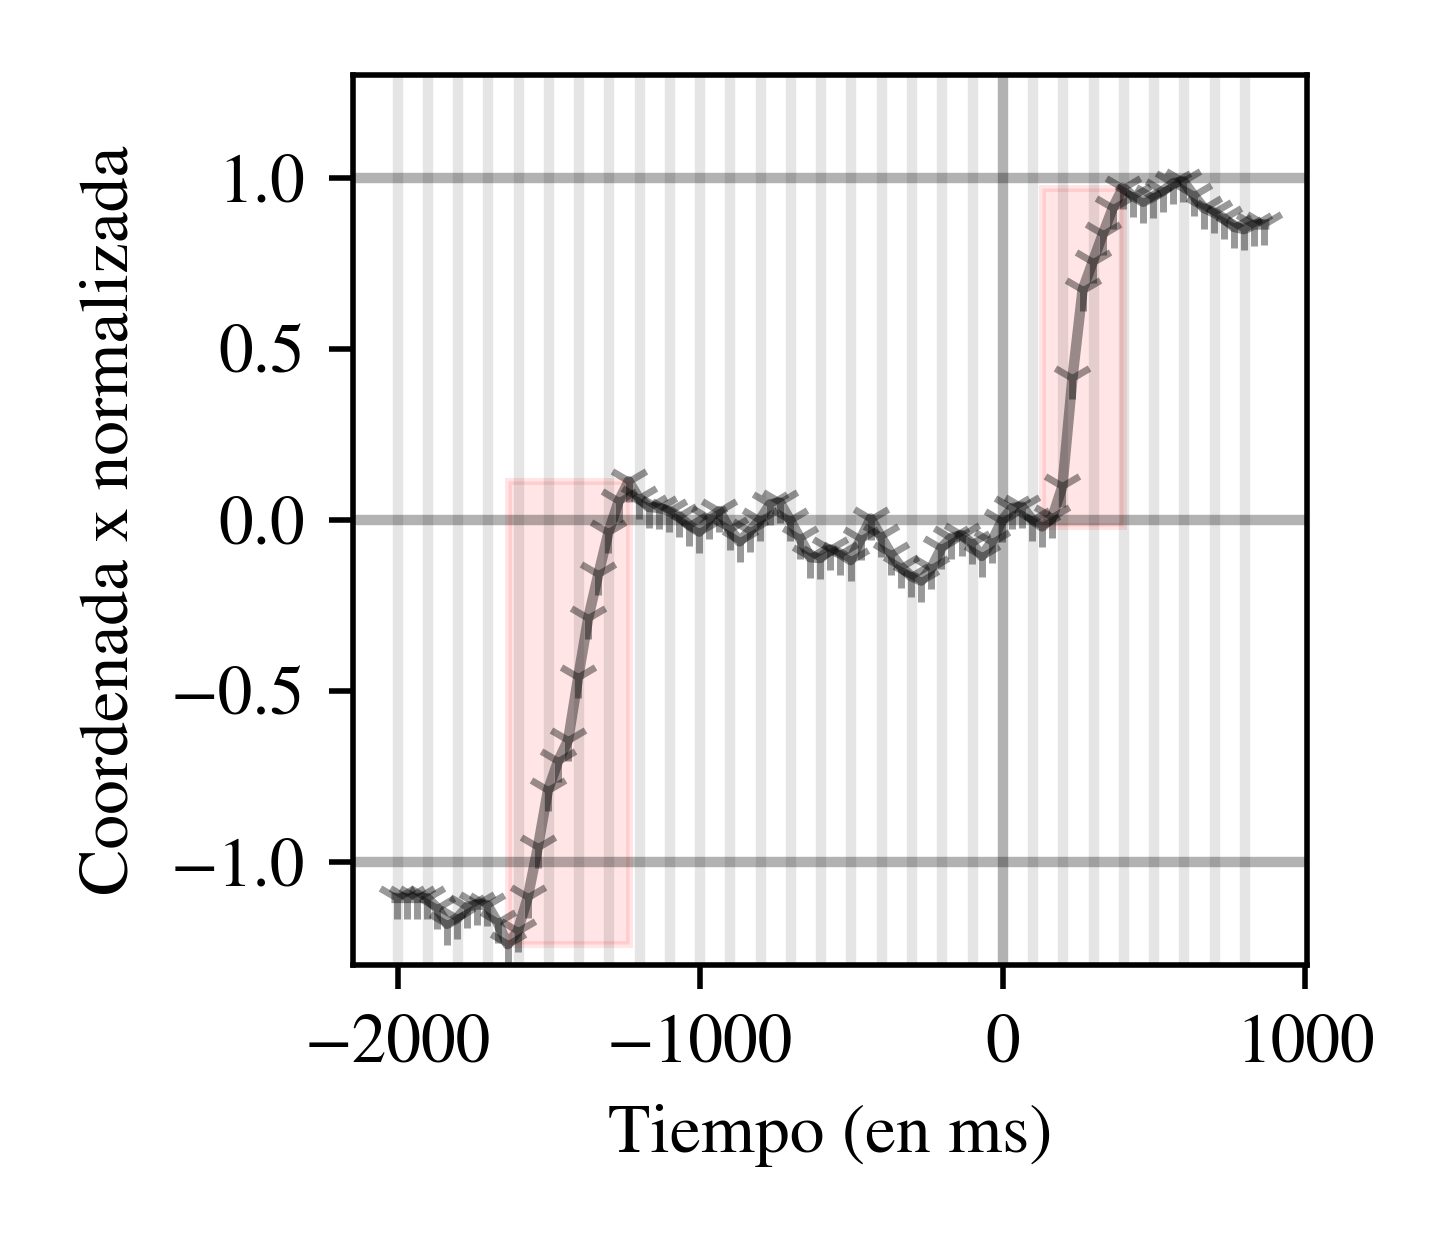
\includegraphics[width=\linewidth]{plots/detected-saccades-example.png}
        \caption{Sacadas detectadas sobre las estimaciones de un ensayo}
      \end{figure}
    \end{column}
  \end{columns}
\end{frame}

\begin{frame}{Conclusiones generales replicadas}
  \begin{table}
    \centering
    \begin{tabular}{ l | c | c | c }
      & correctitud & \multicolumn{2}{ c }{tiempo de respuesta (ms)} \\
      &             & correcto & incorrecto \\
      \hline
      antisacada & 81.29\% & 509 (93) & 346 (105) \\
    \end{tabular}
    \caption{Primera instancia}
  \end{table}
  
  \begin{table}
    \centering
    \begin{tabular}{ l | c | c | c }
      & correctitud & \multicolumn{2}{ c }{tiempo de respuesta (ms)} \\
      &             & correcto & incorrecto \\
      \hline
      antisacada & 94.82\% & 358 (109) & 299 (103) \\
      \hline
      prosacada & 98.09\% & 320 (108) & 311 (150) \\
    \end{tabular}
    \caption{Segunda instancia}
  \end{table}

  % TODO: Poner marker negativo acá
  En la bibliografía para la tarea de antisacadas se reportan \textbf{valores
  de correctitud} más cercanos al rango $[60\%, 75\%]$.
\end{frame}

\begin{frame}{Menos datos de lo esperado}
  \begin{columns}
    \begin{column}{0.4\textwidth}
      \begin{itemize}
        \item Cantidad de ensayos iniciales baja en relación a otros trabajos
        \item Descarte de aproximadamente $\frac{2}{3}$ de los datos
        \item Altas e inesperadas tasas de correctitud
      \end{itemize}
    \end{column}

    \begin{column}{0.6\textwidth}
      \begin{table}
        \centering

        \begin{tabular}{ l | c | c }
          Antisacadas   & incorrecto  & correcto \\
          \hline
          \# total      & 64          & 1173 \\
          \hline
          \# por sujeto & 4.57 (2.84) & 78.20 (40.38)
        \end{tabular}

        \vspace{0.3cm}

        \begin{tabular}{ l | c | c }
          Prosacadas    & incorrecto  & correcto \\
          \hline
          \# total      & 22          & 1134 \\
          \hline
          \# por sujeto & 2.44 (1.23) & 75.59 (38.58)
        \end{tabular}

        \caption{Desbalance entre grupos incorrecto y grupo correcto}
      \end{table}
    \end{column}
  \end{columns}
\end{frame}

\begin{frame}{~}
  fin
\end{frame}

\section{Motivación}

\begin{frame}{~}

  \begin{itemize}
      \item Los ojos como entrada a los procesos cognitivos y estados
        emocionales de una persona
      \item Frecuentemente estudiados en el contexto de la neuropsicología
        digital para estimar el comportamiento
      \item Importante incluso cuando no son el foco del análisis
        (\textit{e.g.}, detección de caras)
      % utilizado también en el desarollo HMI, en el estudio de usabilidad de
      % interfaces, recientemente en el campo de la oftalmología para estimar
      % el campo visual
      \item Usos en otras disciplinas
  \end{itemize}

  \begin{figure}
    \begin{subfigure}{0.49\textwidth}
      \centering
      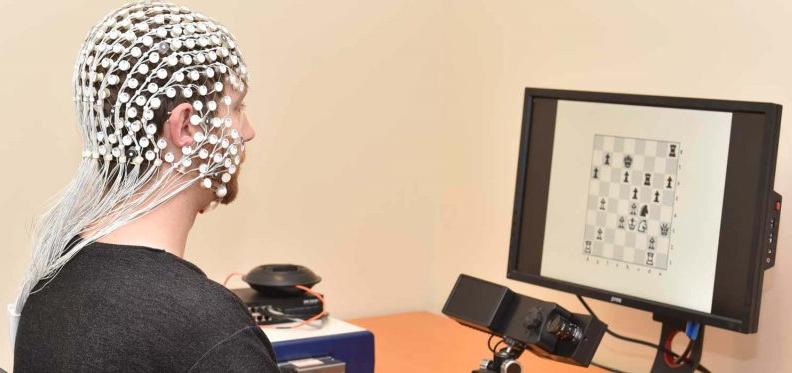
\includegraphics[width=\linewidth]{img/eye-link-eeg.jpg}
      \caption{\textit{Eye tracking} combinado con electroencefalograma}
    \end{subfigure}
    \begin{subfigure}{0.49\textwidth}
      \centering
      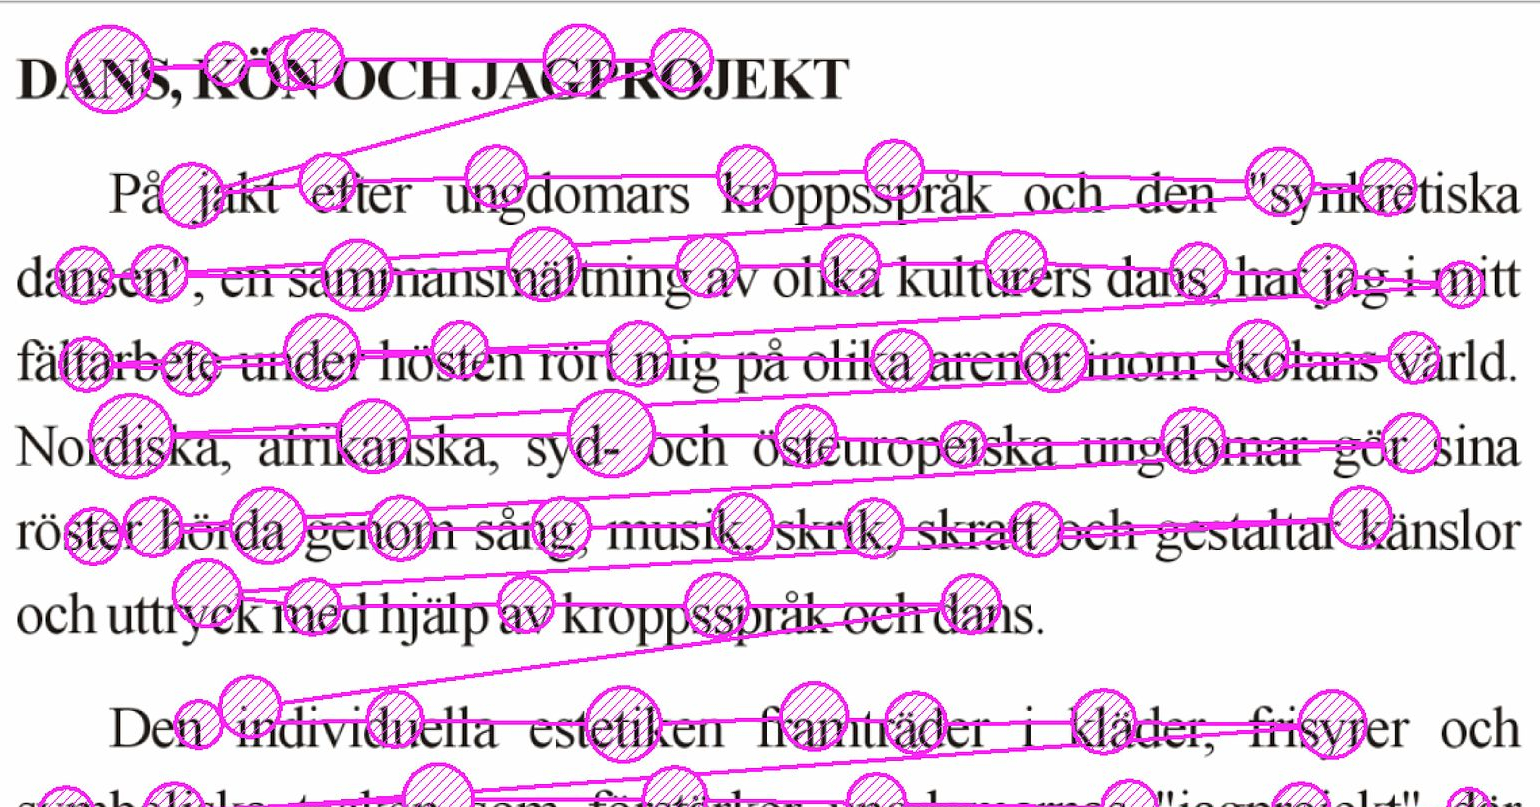
\includegraphics[width=\linewidth]{img/reading-fixations-saccades.jpg}
      \caption{Estimación de la mirada durante una tarea de lectura}
    \end{subfigure}
  \end{figure}

\end{frame}

\begin{frame}{~}

  \begin{itemize}
    \item Comunmente resuelto con sistemas comerciales cerrados
    \item Costos altos (entre 5000 y 40000 euros) mientras que el hardware en
      sí representa una pequeña fracción de estos (entre 200 y 600 euros)

    % si falta algún dato (e.g., la precisión del diámetro de la pupila) no
    % se lo puede saber
    \item Imposibilidad de auditar la implementación
    \item Necesidad de asistir a un laboratorio
  \end{itemize}

  \begin{figure}
    \begin{subfigure}{0.49\textwidth}
      \centering
      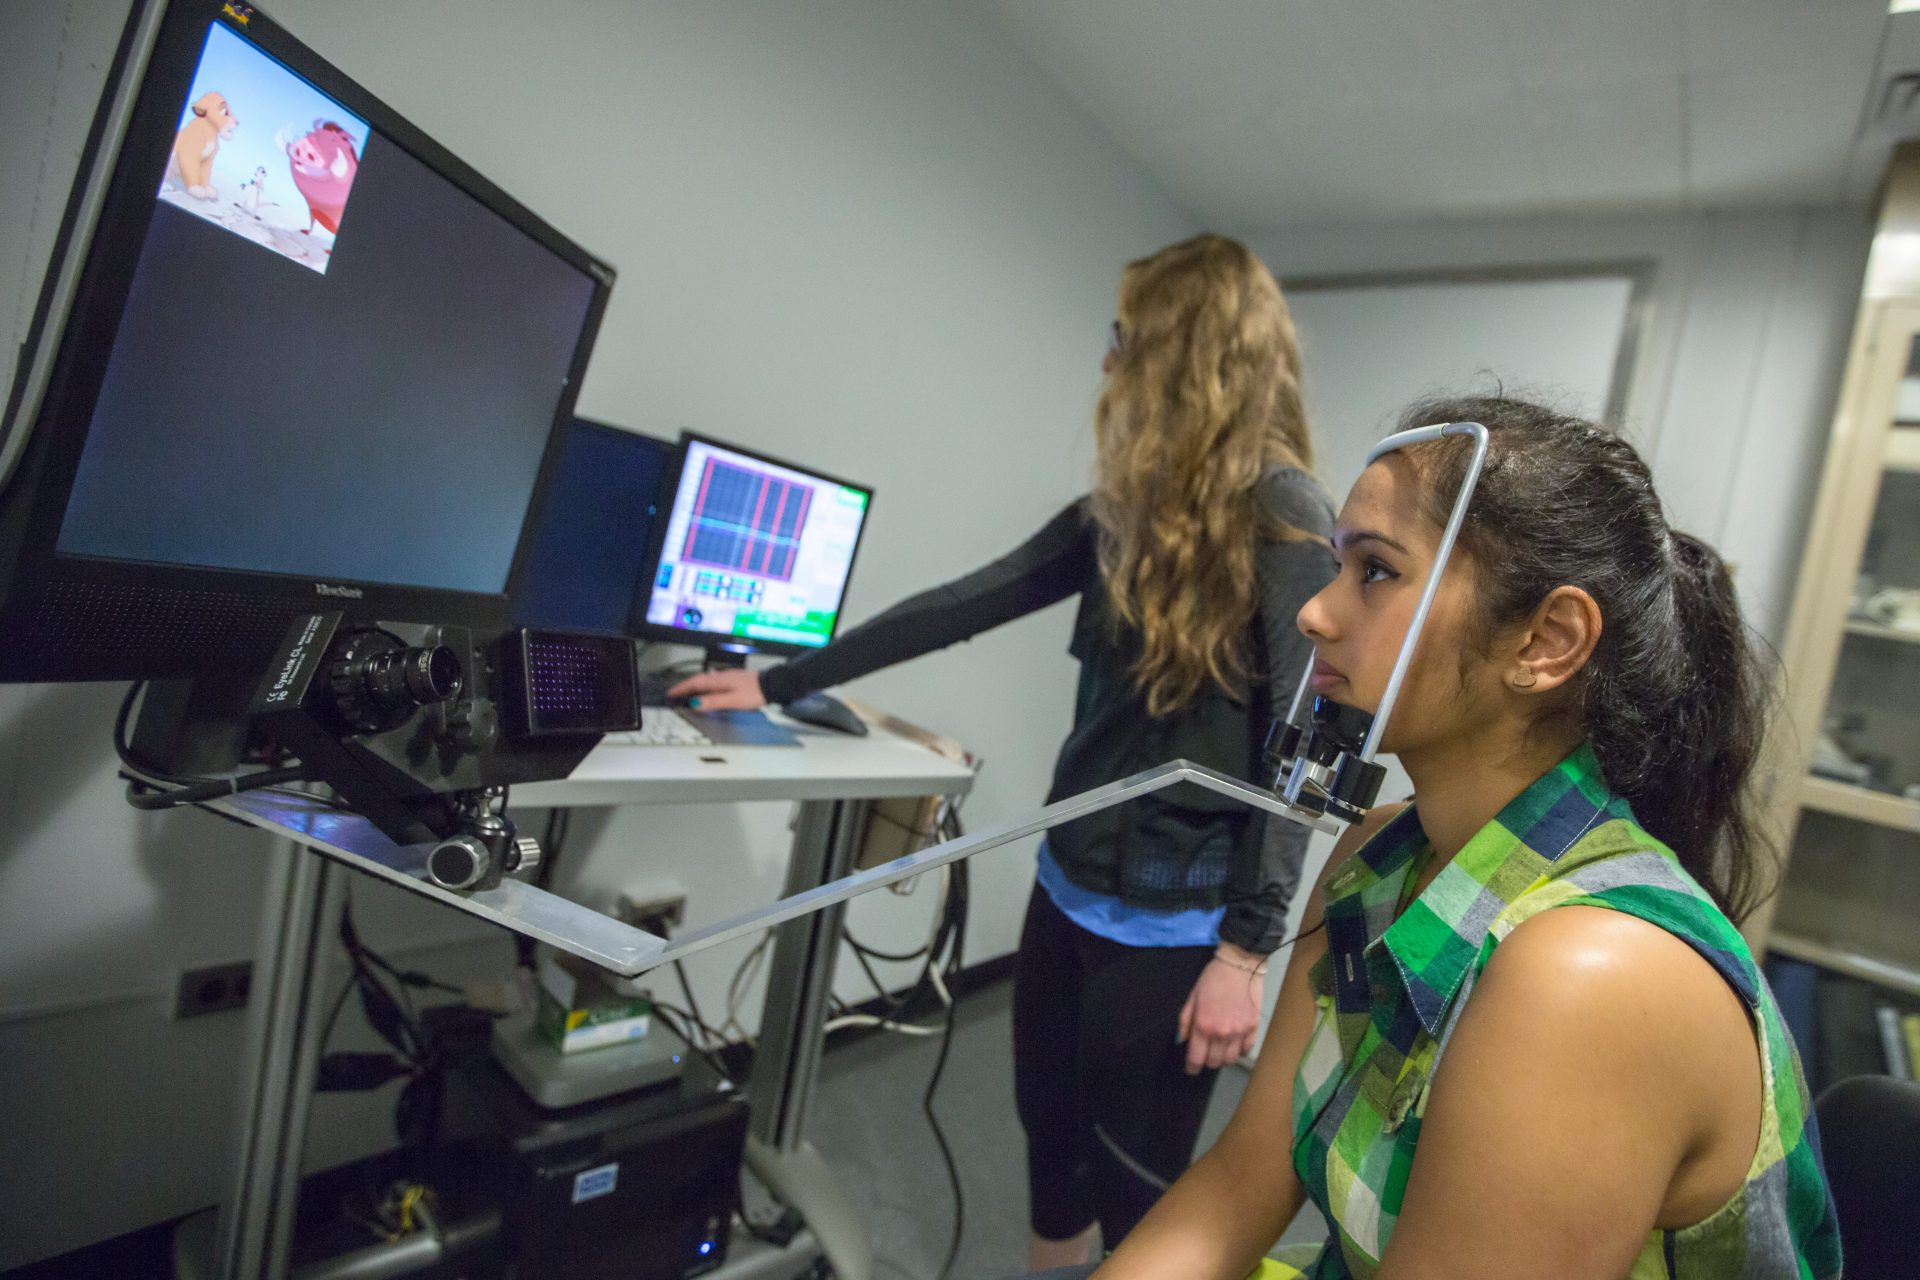
\includegraphics[width=0.6\linewidth]{img/eye-link-chinrest.jpg}
      \caption{La reestricción de movimiento facilita mantener calibrado el
      sistema}
    \end{subfigure}
    \begin{subfigure}{0.49\textwidth}
      \centering
      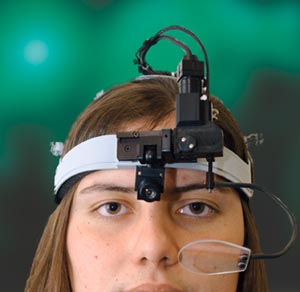
\includegraphics[width=0.5\linewidth]{img/eye-tracker-head-mounted.jpg}
      \caption{\textit{Eye tracker} montado a la cabeza}
    \end{subfigure}
  \end{figure}

\end{frame}

\begin{frame}{~}

  \begin{columns}
    \begin{column}{0.4\textwidth}
      \begin{itemize}
        \item Interés en proveer software de \textit{eye tracking}

        \item Posibilidad de \textit{crowdsourcing}

          % e.g., detectar pérdidas de atención en clases masivas
        \item Potencial para nuevas aplicaciones
      \end{itemize}

    \end{column}
    \begin{column}{0.6\textwidth}

      \begin{figure}
        \begin{subfigure}{0.49\textwidth}
          \centering
          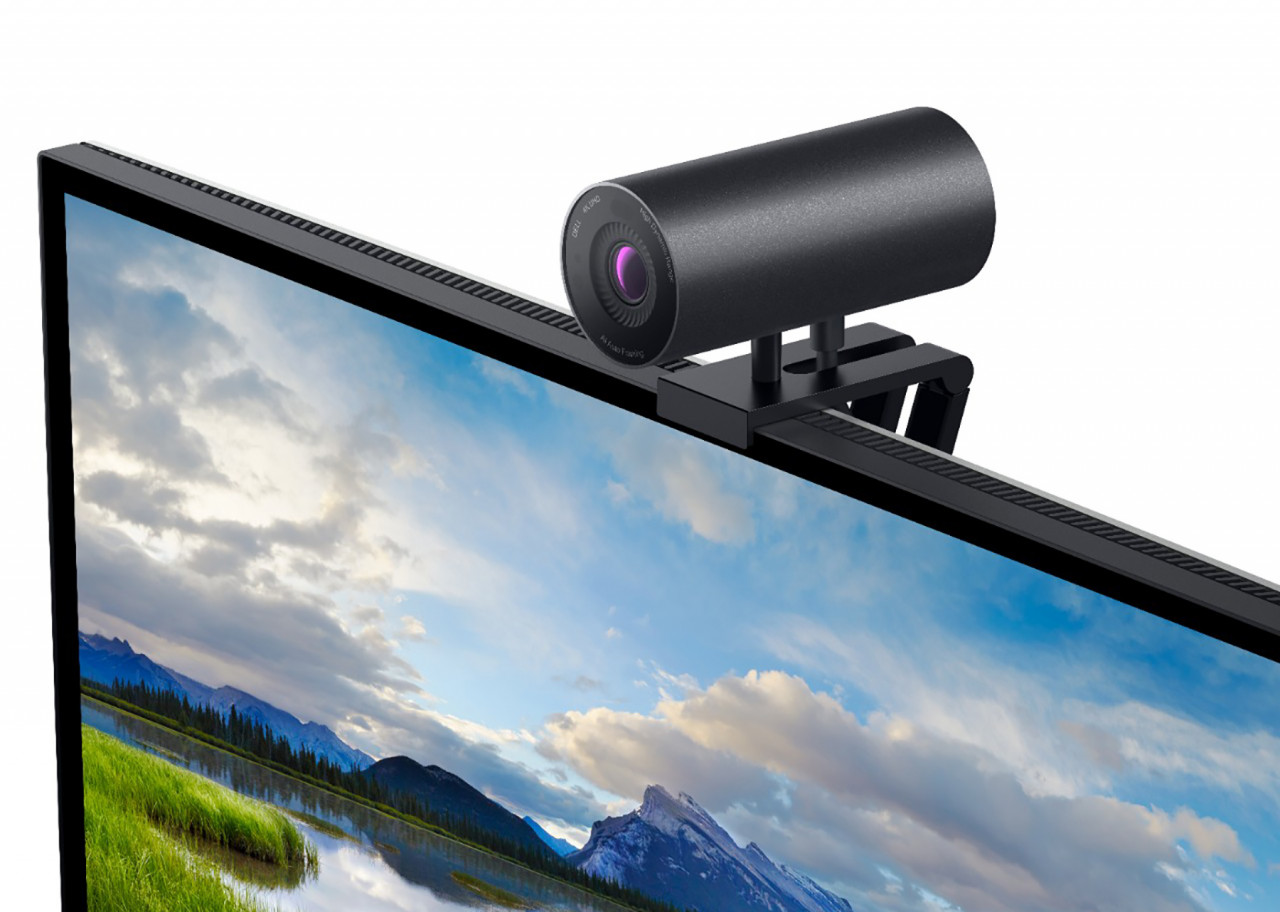
\includegraphics[width=0.8\linewidth]{img/external-webcam.jpg}
        \end{subfigure}
        \begin{subfigure}{0.49\textwidth}
          \centering
          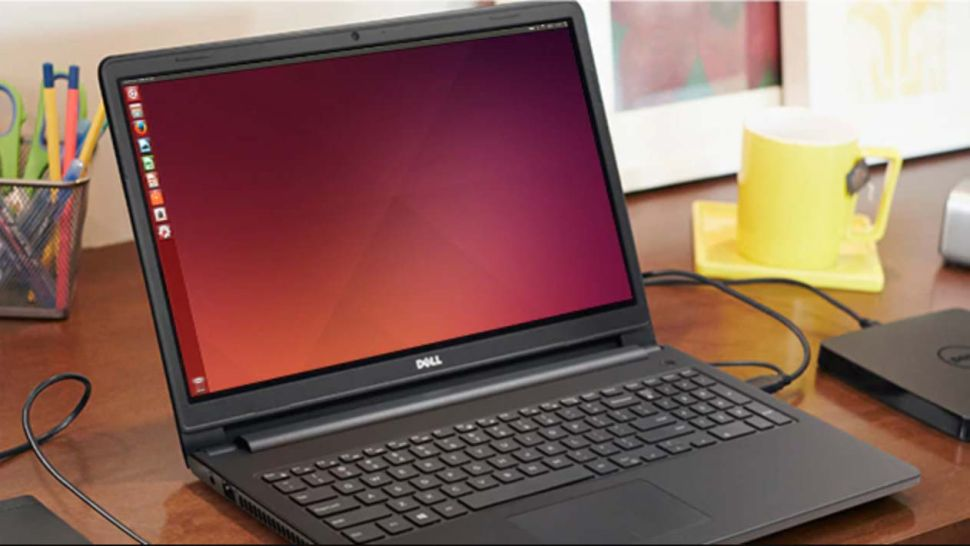
\includegraphics[width=0.8\linewidth]{img/notebook.jpg}
        \end{subfigure}
        \caption{Webcams domésticas ya disponibles}
      \end{figure}

      \begin{figure}
        \begin{subfigure}{0.49\textwidth}
          \centering
          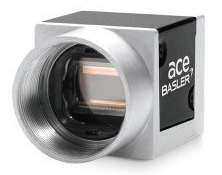
\includegraphics[width=0.6\linewidth]{img/basler-camera.jpg}
        \end{subfigure}
        \begin{subfigure}{0.49\textwidth}
          \centering
          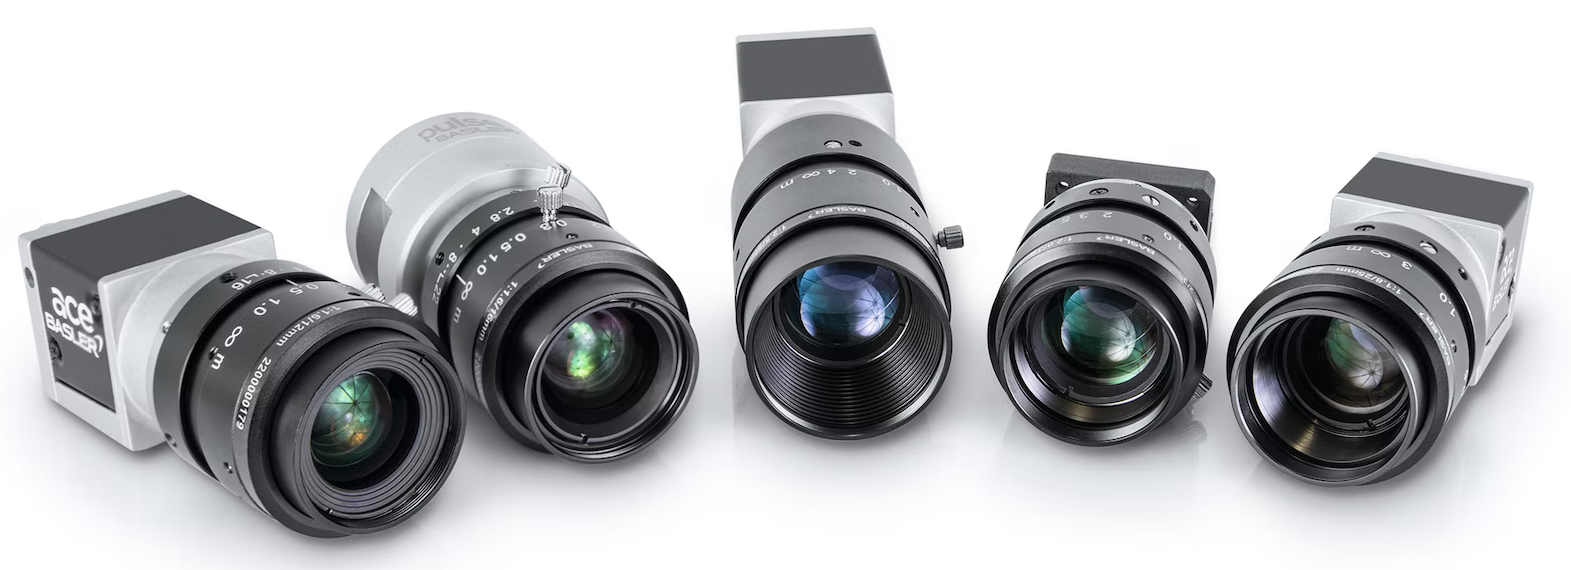
\includegraphics[width=0.8\linewidth]{img/basler-cameras-with-lens.png}
        \end{subfigure}
        \caption{Hardware profesional adquirible por una fracción del costo}
      \end{figure}


    \end{column}
  \end{columns}
\end{frame}

\section{Objetivos}

\begin{frame}{~}

  \begin{itemize}
    \item Evaluar implementaciones recientes con similares motivaciones
    % - entender el problema
    % - definir los requerimientos
    % - establecer qué puede reutilizarse

    \item Implementar un prototipo de \textit{eye tracker} que corra en
      navegadores \textit{web} y que esté orientado a análisis clínicos
    % - adaptar lo que pudiera reutilizarse
    % - implementar los módulos que faltaran

    \item Emular análisis clínicos remotos y recolectar datos utilizando el
      prototipo implementado

    \item Establecer la capacidad del prototipo en replicar conclusiones
      establecidas con \textit{eye trackers} profesionales de laboratorio

  \end{itemize}

\end{frame}

\section{Desarmando el problema de \textit{eye tracking} web}

\begin{frame}{~}
  \begin{columns}
    \begin{column}{0.5\textwidth}
      \begin{itemize}
        \item Estimar qué coordenada de la pantalla está mirando el usuario en
          un contexto de estudios clínicos
        \item Un \textit{stream} de frames de la webcam como \textit{input}
        \item Se divide en \textbf{localizar los ojos} y luego \textbf{estimar
          la mirada}
        \item Calibraciones necesarias en cada sesión de uso
      \end{itemize}
    \end{column}
    \begin{column}{0.5\textwidth}
      \begin{figure}
        \centering
        TODO: Reemplazar esto por un único plot que ejemplifique el output
        deseado
        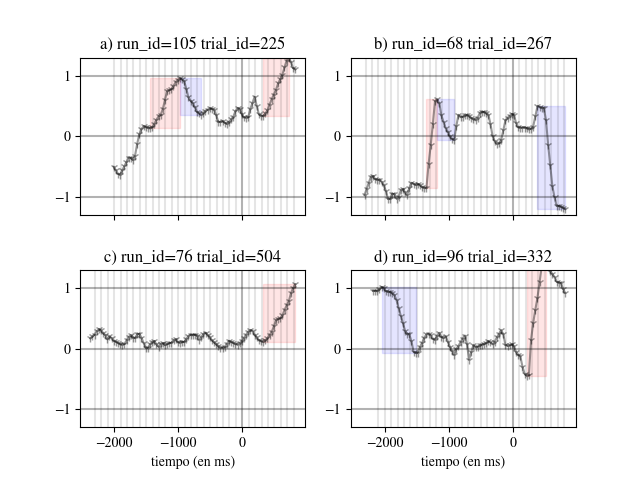
\includegraphics[width=\linewidth]{img/eye-tracking-output-example.png}
        \caption{Sacadas detectadas sobre serie de tiempo de la coordenada x}
      \end{figure}
    \end{column}
  \end{columns}
\end{frame}

\begin{frame}{~}
    \begin{itemize}
    \item Resultados consistentes dentro de una misma población
    % - mayor tasa de correctitud para los casos de prosacada que para aquellos de antisacada
    % - para los grupos correctos se esperan mayores tiempos de respuesta en las repeticiones de antisacadas que en aquellas de prosacadas
    % - a mayor edad menor rendimiento en la tarea, tanto en latencia como en correctitud

    \item Búsqueda de establecer resultados para poblaciones de distinta condición neuropsicológica
    % - ditintos tipos de lesiones cerebrales
    % - déficit de atención, esquizofrenia, síndrome de Parkinson, síndrome de Tourette
    % - individuos sanos, efectos de la edad

    \item Comparación dificultosa entre distintos trabajos
    % - se obtienen valores del mismo orden (RT y correctitud) para pacientes sanos en un estudio que para pacientes con esquizofrenia de otro estudio
    \end{itemize}

\end{frame}

\section{Alternativas al \textit{eye tracking} tradicional}

\subsection{Trabajos previos}

\begin{frame}{~}

  TODO: Separar esto en varios frames
  \begin{itemize}
    \item \texttt{PupilEXT}: software para realizar pupilometría; deben
      proveerse cámaras profesionales y emisores de luz infrarroja; TODO:
      imagen pupilometría

    % hay que resaltar la importancia de esto de analizar el momento de mayor
    % coincidencia
    \item \texttt{PACE}: aplicación de escritorio basada en webcam; calibran en
      base a interacciones del usuario; analizar el momento de mayor
      coincidencia entre la mirada y la posición de la interacción; TODO:
      alguna imagen del paper

    \item \texttt{TurkerGaze}: aplicación web basada en webcam; generación de
      mapas de saliencia a través de \textit{crowdsourcing}; TODO: imagen mapas
      de saliencia

    \item \texttt{WebGazer}: aplicación web basada en webcam; se basan en
      \texttt{PACE} y \texttt{TurkerGaze}; provisto en forma de paquete; TODO:
      screenshot del paquete

  \end{itemize}

\end{frame}

\subsection{Implicancias del contexto remoto de navegador \textit{web}}

\begin{frame}{~}

  \begin{itemize}
    \item[+] Posibilidad de reutilizar cámaras web

    \item[+] Compatibilidad con otras herramientas web, en particular
      \texttt{JSPsych}

    % no es el fin del mundo pero es un lenguaje bastante odiado e implica
    % dificultades en cuanto a la precisión. Por ejemplo, la duración de cada
    % frame va a ser variable, lo que dificulta mostrar estímulos durante
    % cortas cantidades de tiempo
    \item Necesidad de implementar sobre JavaScript

    % no sólo las webcams son variables si no que tmb la compu donde corre el 
    % programa
    \item[--] Hardware variable de potencialmente bajo rendimiento

    % deben transmitirse en texto e imagenes sin que puedan hacerse
    % aclaraciones en el momento. esto implica una duración total del
    % experimento potencialmente mayor
    \item[--] Las instrucciones no pueden ser transmitidas en persona

    % puede variar la luz o la disposición del hardware
    \item[--] Ambiente físico no controlado
  \end{itemize}

  TODO: Screenshots de JSPsych y de Amazon Mechanical Turk

\end{frame}

\subsection{Modelado de la mirada}

\begin{frame}{~}
  \begin{itemize}
    % no entrar en detalle con esto pero mencionar brevemente por qué
    \item Limitados a una pequeña fracción de la bibliografía debido a tener
      una y sólo una cámara
    
    % acuerdo en que hay que mostar una serie de puntos pero no está claro
    % cuántos, ni cómo, ni qué información rescatar. tmb hay interés en
    % minimizar la duración del exp
    \item Falta de estándar respecto de cómo calibrar

    % ante ligeros movimientos de cabeza el sistema va a quedar descalibrado.
    % hay que tenerlo en cuenta en el flow del experimento. puede recalibrarse
    % cada un tiempo fijo (TG), agregar data de calibración a medida que avanza
    % el experimento (WG) o bien implementarse alguna heurística para decidir
    % cuándo el sistema necesita una recalibración
    \item Ausencia de invarianza frente a movimientos de cabeza y de
      reestricción de movimiento
  \end{itemize}
\end{frame}

\section{Implementación}

\section{Experimentación}

\section{Resultados}

\subsection{Características de los datos}

\begin{frame}{Frecuencias de muestreo}

  TODO: Acomodar subplots y mostrarlo solo por estimaciones para que sea menos
  lío
  \begin{figure}
    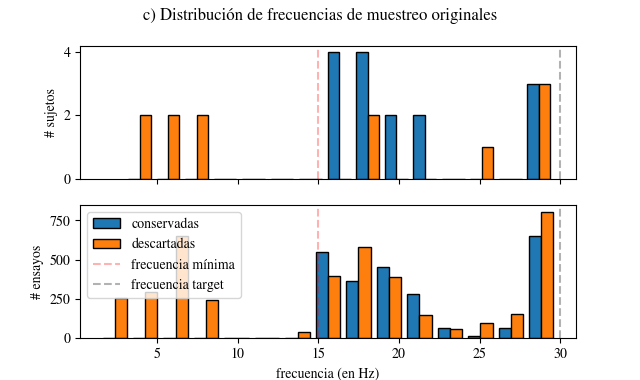
\includegraphics[width=0.7\linewidth]{img/second-sampling-frequencies-distribution.png}
  \end{figure}

\end{frame}

\begin{frame}{Anchos de pantalla}

  TODO: Acomodar subplots y mostrarlo solo por estimaciones para que sea menos
  lío
  \begin{figure}
    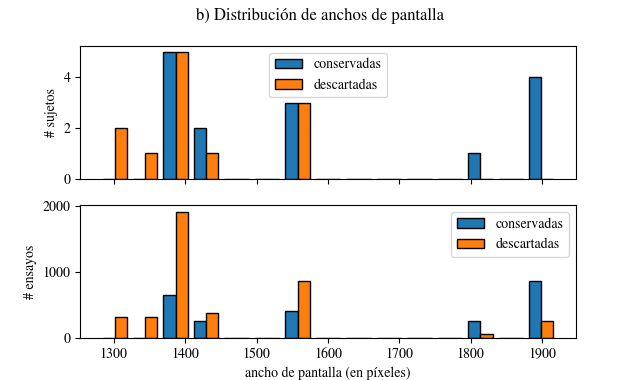
\includegraphics[width=0.7\linewidth]{img/second-widths-distribution.png}
  \end{figure}

\end{frame}

\begin{frame}{Estimaciones desviadas}

  TODO: Acomodar subplots
  \begin{figure}
    \includegraphics[width=0.8\linewidth]{img/skewed-estimations-examples.png}
  \end{figure}

\end{frame}

\subsection{Limpieza y normalización}

\subsection{Detección de sacadas}

\begin{frame}{~}

  Luego de normalizar, se considerará un intervalo como una sacada si:
  \begin{enumerate}
    \item La mirada se mueve en una misma dirección
    \item El intervalo dura al menos 40 ms
    \item Se recorre \textit{cierta} distancia mínima durante ese intervalo
    \item El desplazamiento es lo \textit{suficientemente rápido}
  \end{enumerate}
  Implementación \textit{ad hoc} cuya calidad no fue estudiada.

\end{frame}

\subsection{Conclusiones generales replicadas}

\begin{frame}{~}
  \begin{columns}
    \begin{column}{0.5\textwidth}
      \begin{figure}
        \centering
        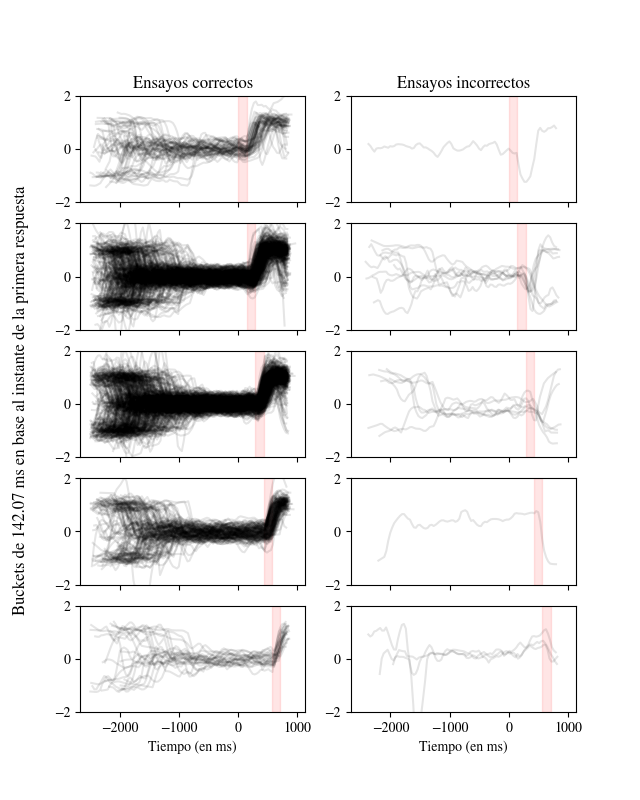
\includegraphics[width=\linewidth]{img/second-disaggregated-prosaccades.png}
      \end{figure}
    \end{column}
    \begin{column}{0.5\textwidth}
      \begin{figure}
        \centering
        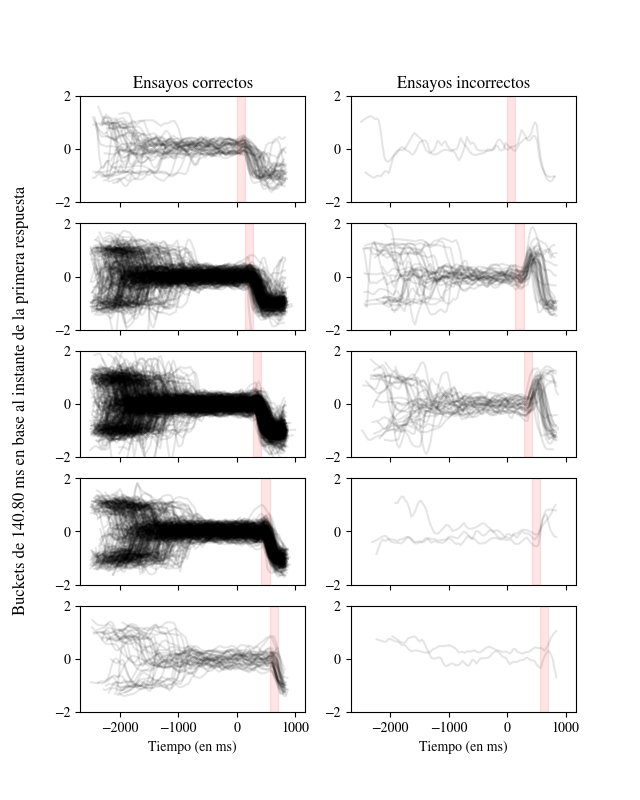
\includegraphics[width=\linewidth]{img/second-disaggregated-antisaccades.png}
      \end{figure}
    \end{column}
  \end{columns}
\end{frame}

\subsection{Grupos etarios no representados}

\begin{frame}{~}
  TODO: Cambiarlo para que sólo muestre los sujetos y no los ensayos
  \begin{columns}
    \begin{column}{0.5\textwidth}
  \begin{figure}
    \centering
    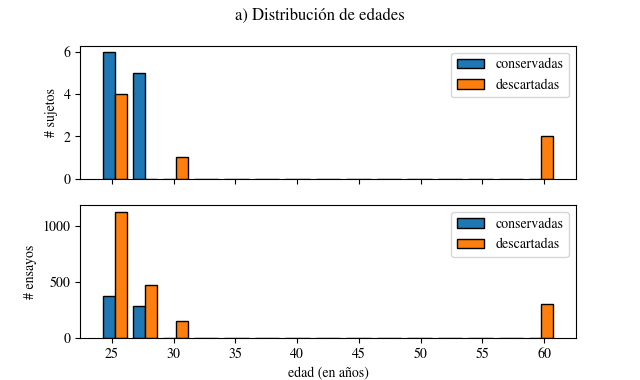
\includegraphics[width=\linewidth]{img/first-ages-distribution.png}
    \caption{Primera instancia}
  \end{figure}
      
    \end{column}
    \begin{column}{0.5\textwidth}
  \begin{figure}
    \centering
    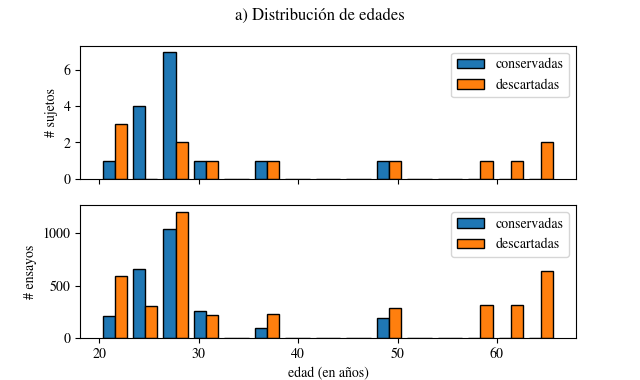
\includegraphics[width=\linewidth]{img/second-ages-distribution.png}
    \caption{Segunda instancia}
  \end{figure}
    \end{column}
  \end{columns}
\end{frame}

\subsection{Menos datos de lo esperado}



\section{Conclusiones}

\begin{frame}{~}
  \begin{itemize}
    \item Se obtuvo un prototipo de \textit{eye tracker} para navegadores web
    \item Potencial para realizar análisis clínicos remotos
    \item Campo aún en sus primeros pasos
    \item Precisión muy por debajo de aquella alcanzable por \textit{eye
      trackers} profesionales
  \end{itemize}
\end{frame}

\subsection{Limitaciones}

\begin{frame}{Implementativas}
  TODO: Las limitaciones y trabajo futuro no ponerlas todas y en cambio referir
  a la tesis \par

. bajas frecuencias
. pestañeos
. estimación del tamaño de la pantalla
. imprecisión en la duración de cada frame, problemático si se quiere mostrar
  un estímulo durante una corta duración de tiempo

  \begin{figure}
    \centering
    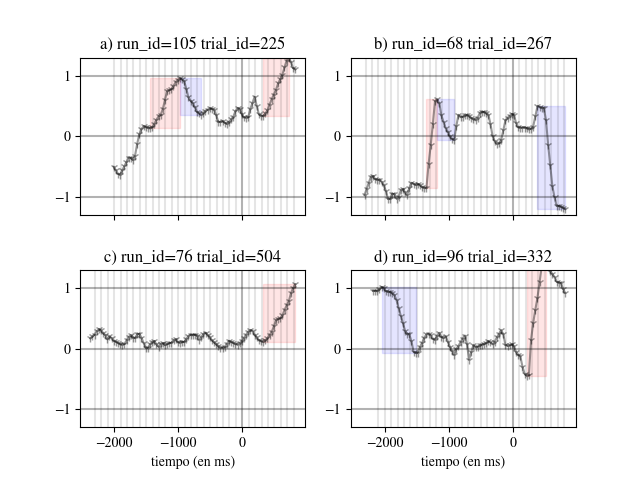
\includegraphics[width=0.9\linewidth]{img/undetected-saccades-examples.png}
    \caption{Ejemplos de sacadas no detectadas}
  \end{figure}
\end{frame}

\begin{frame}{Experimentales}
. proporción de datos filtrados demasiado elevada
. necesidad de revisar la causa de las altas tasas de correctitud obtenidas
. representatividad de distintos grupos etarios
\end{frame}

\subsection{Trabajo futuro}

\begin{frame}{Análisis de datos}
. Investigar e implementar mecanismos estándares de detección de sacadas, lo
  cual podría basarse en la previa construcción de un dataset etiquetado de
  sacadas
. Revisar criterios de exclusión para asegurarse de no estar filtrando datos
  válidos
. Realizar nuevas rondas de experimentación, estimando previamente la cantidad
  de ensayos necesarios para asegurar cantidades suficientes en los grupos
  incorrectos y en los distintos grupos etarios
\end{frame}

\begin{frame}{Análisis de sensibilidad}
. propuesta sobre experimento para recolectar datos y establecer métricas de
  calidad sobre las estimaciones obtenidas por la herramienta
TODO: Acá combinar un poco lo que quedó en la tesis y lo que pensé para
      sensitivity analysis
\end{frame}

\begin{frame}{Prototipo desarrollado}
. optimizar frecuencia de muestreo
. reexplorar detección de descalibraciones y qué significa que el sistema esté
  descalibrado
. mejorar la calibración, generalizarla a más puntos de interés
. detección de pestañeos
. estimación del tamaño de la pantalla y posibilidad de mostrar estímulos en
  grados
. verificación de condiciones iniciales
TODO: Extender con lo que haya escrito en la tesis
\end{frame}

\begin{frame}{\textit{Eye tracking} en navegadores \textit{web}}
. extender bibliografía que aplique a nuestro contexto
. eye tracking web no podría atacar algunos problemas que sí puede el eye
  tracking tradicional, pero al ser remoto y de bajo costo es posible que
  permita atacar nuevos problemas. Deben entonces buscarse tales problemas
\end{frame}

\end{document}


\chapter{Desarrollo}

\section{Método}

\subsection{Implementación}

Se construyó un prototipo de \eyetracker web formado por módulos preexistentes
y desarrollos propios.
El contexto remoto no supervisado explicado previamente tiene implicaciones
sobre su implementación.
Este debe funcionar en un navegador web, y en particular debe ser compatible
con la herramienta de experimentos conductuales \jspsych. 
l sujeto no contará con alguien que lo supervise durante el experimento ni con
una estructura que le ayude a mantener la cabeza quieta.
Por lo tanto se deberá definir algún criterio que nos indique cuándo es
necesaria una recalibración.

Se implementó entonces una herramienta que provee una estimación de la mirada
con fases explícitas de calibración, verificando a lo largo del tiempo si el
sujeto movía la cabeza respecto de su posición durante la calibración.
De \webgazer se reutilizó principalmente su modelo de estimación de la mirada y
utilidades como aquella que muestra en la pantalla la coordenada estimada de la
mirada.
Sin embargo, se descartó utilizar sus elementos de calibración pues no aplican
a nuestro caso.
Además, se mantuvo una división explícita entre el código correspondiente al
\eyetracking (el \textit{core}) respecto de la interfaz con \jspsych.
Al prototipo implementado se le dio el nombre \rastoc para poder referirse a él
dentro del código.

\begin{figure}
    \centering
    \includegraphics[width=0.8\linewidth]{media/components.png}
    \caption{Relaciones entres componentes implementados y componentes
    existentes}
    [TODO: Poner línea punteada a los componentes propios]
    \label{fig:components}
\end{figure}

\subsubsection{Calibración}

La calibración del sistema consiste en acumular un conjunto de pares
$<$\textit{features} de los ojos, coordenada$>$.
Cada uno de estos pares representa a qué coordenada de la pantalla estaba
mirando el sujeto cuando la imagen de sus ojos tenía un determinado aspecto.
Las \textit{features} utilizadas incluyen las coordenadas y dimensiones del
recuadro capturado en relación al \textit{frame} entero, así como un vector
correspondiente al recuadro en sí como una imagen.
La conversión de \textit{frames} a \textit{features} es realizada continuamente
por \webgazer (cf. estimación de la mirada).

La construcción del conjunto de calibración se hará en base a una secuencia de
interacciones por parte del sujeto.
Al momento de tal interacción se guardará el par formado por el último
\textit{frame} capturado y la coordenada de la interacción.
Esto puede hacerse únicamente luego de iniciar una fase explícita de
calibración.
La Figura \ref{fig:calibration_cycle} ilustra las distintas etapas de
calibración recorridas por el sistema.
Al finalizar esta etapa el conjunto acumulado se utiliza para: a) entrenar el
modelo de regresión utilizado por \webgazer para estimar la mirada; b)
instanciar el mecanismo de detección de movimiento.

\begin{figure}
    \centering
    \includegraphics[width=0.8\linewidth]{media/calibration_cycle.png}
    \caption{Posibles estados de calibración del prototipo implementado}
    En los estados con linea punteada el sistema no podrá realizar estimaciones
    de la mirada.
    Notar que se continuará dando estimaciones incluso cuando se considere que
    el sistema se ha descalibrado.
    Los distintos mecanismos de calibración se adaptan a este esquema y
    difieren en cómo el usuario realiza el mapeo coordenada a \textit{frame}.
    \label{fig:calibration_cycle}
\end{figure}

Al iniciar una fase explícita de calibración, el \textit{core} provee dos
métodos para indicar tales coordenadas.
El primero (\texttt{calibrationType === “click”}) permite al experimentador
indicar que cada click realizado en la pantalla tendrá que ser usado para
calibrar el sistema.
El segundo (\texttt{calibrationType === “external”}) devuelve un
\textit{callback} que el experimentador podrá utilizar cuando lo desee,
permitiéndole entonces implementar el mecanismo de calibración que prefiera.
Se asume siempre que el sujeto estará mirando a la coordenada input.

A nivel \jspsych, a través de estos dos mecanismos se ofrecen dos opciones
distintas que el experimentador puede utilizar para que el sujeto calibre el
sistema.
Por un lado, está la calibración libre, en la cual el sujeto tendrá que
clickear en la pantalla mientras mira el puntero.
Por otro lado está la calibración asistida, que funciona a través del paquete
\psychophysics [0.2] y durante la cual se dibujan una serie de estímulos en la
pantalla, ilustrado en la Figura \ref{fig:calibration_stimulus}.
Cada vez que aparece uno de estos, el sujeto tendrá que fijar la mirada en él y
presionar la barra de espacio para indicar que lo está mirando.
Buscando minimizar la cantidad de puntos mostrados, esta calibración prioriza
asegurar buenas estimaciones únicamente en las regiones de interés, que en el
caso de la tarea de antisacadas son tres.
Para esto se eligen mostrar estímulos de calibración sobre un eje horizontal
central en el centro, en la derecha y en la izquierda.

\begin{figure}
    \centering
    \includegraphics[width=0.4\linewidth]{media/calibration-stimulus-left.png}
    \includegraphics[width=0.4\linewidth]{media/calibration-stimulus-center.png}
    \includegraphics[width=0.4\linewidth]{media/calibration-stimulus-right.png}
    \caption{Estímulos de calibración}
    Al realizar una calibración asistida el sujeto es presentado con estímulos
    visuales en las regiones de interés.
    Para avanzar con la calibración, el sujeto deberá fijar la mirada en cada
    estímulo que aparece y luego presionar la barra de espacio. \\
    \label{fig:calibration_stimulus}
\end{figure}

Finalizada la etapa explícita de calibración, el sistema puede recalibrarse
cuando se considere necesario.
Para esto debe iniciarse una nueva fase de calibración explícita que
reemplazará los datos de la calibración anterior.

\subsubsection{Validación}

La interfaz \jspsych provee la opción de realizar una validación luego de cada
calibración.
En esta se muestran progresivamente estímulos en el centro y en las cuatro
esquinas de la pantalla.
Al igual que con la calibración asistida, cada vez que aparezca un estímulo, el
sujeto deberá fijar la mirada en él y presionar la barra de espacio.
Durante la presentación de estos estímulos se estará estimando la mirada en la
pantalla.
Idealmente se verificaría que durante un período previo a la interacción del
sujeto estas estimaciones coincidan en algún grado con las coordenadas de los
estímulos presentados \cite{huang_2016_pace}.
Sin embargo, debido a las desviaciones detectadas en la primer fase de
experimentación (cf. sección \ref{section:skewed-estimates}) se
verifica, en cambio, un correcto posicionamiento relativo.
Dicho de otra manera, en lugar de verificar que al mostrar un estímulo en la
esquina superior derecha las estimaciones coinciden con la coordenada de tal
estímulo, se verificará en cambio que tales estimaciones están a la derecha de
las estimaciones obtenidas al mostrar el estímulo superior izquierdo.
Debido a lo ya mencionado respecto de los mecanismos de calibración (cf.
sección \ref{section:intro:calibration}) y a que en este trabajo no interesa
analizar las coordenadas verticales de las estimaciones (pues implementamos
únicamente la tarea de antisacada) se optó además por verificar únicamente que
hubiera un correcto posicionamiento relativo horizontal.
Queda pendiente estudiar e implementar mecanismos de calibración y validación
que balanceen correctamente experiencia de uso y calidad de las estimaciones.

Como se detallará en la sección de preprocesamiento (sección
\ref{section:preprocessing}), este mecanismo de validación facilita luego la
implementación de una rutina de normalización.

\subsubsection{Estimación de la mirada}

Se delegó la estimación de la mirada al paquete \webgazer
\cite{papoutsaki_2016_webgazer}.
Esta se basa en un modelado explícito de la cara para localizar los ojos y un
modelo por apariencia para estimar la mirada.

La localización de los ojos se realiza a través del modelo de \textit{facemesh}
de \texttt{TensorFlowJS}
\footnote{\url{https://github.com/tensorflow/tfjs-models/tree/master/face-landmarks-detection}}.
Utilizando los \textit{keypoints} obtenidos se recorta de cada \textit{frame}
un recuadro para cada ojo.
No está claro si este mecanismo es ideal pues, por ejemplo, se está modelando
toda la cara mientras que nos importa únicamente la posición de un par de
recuadros de los ojos.
No sólo parece excesivo en términos de costos computacionales, si no que al no
estar modelando específicamente los ojos sería esperable no obtener la mejor
precisión que podría obtenerse.
Existen en cambio mecanismos específicos para la localización de los ojos
\cite{hansen_2009_eye_of_the_beholder}.

Cada recuadro tiene luego su tamaño ajustado a una dimensión fija de 10x6
píxeles.
Se los convierte luego a una escala de grises y son ecualizados a través de
histogramas.
De esta manera, para cada \textit{frame} de la webcam se obtiene un vector de
120 dimensiones correspondiente a la apariencia de los dos ojos.
De este universo 120D se pasa luego al universo de coordenadas 2D a través de
un modelo de \textit{ridge regression}.
Los coeficientes de este modelo se calculan al finalizar la fase explícita de
calibración.

\subsubsection{Descalibración}

A modo de primer acercamiento se implementó un mecanismo basado en detectar
movimiento de los ojos del sujeto.
En base al conjunto de \textit{features} de ojos capturados al calibrar, se
obtienen un par de conjuntos de rectángulos que contienen a los ojos en cada
uno de los correspondientes \textit{frames}.

Se definen luego, para cada ojo, un multipoligono (i.e., una forma geométrica
definida en base a múltiples polígonos) correspondiente a la unión de los
rectángulos de cada ojo, agrandados luego por un factor de 1.8 (elección
arbitraria basada en experimentación al desarrollar el prototipo).
El multipoligono obtenido para cada ojo representa el espacio dentro del cual
el recuadro del ojo deberá mantenerse para que se considere que no hubo
movimiento significativo.
Si a partir de algún \textit{frame} el recuadro de alguno de los ojos sale de
su multipoligono se considerará al sistema como descalibrado.

\subsubsection{Playgrounds}

Para ambas interfaces implementadas se construyó también un \textit{playground}
que permitiera interactuar con ellas.
El del \textit{core} (Figura \ref{fig:rastoc-playground}) permite realizar
calibraciones libres y visualizar la coordenada estimada de la mirada en la
pantalla al mismo tiempo que imprime ciertos datos de la calibración.
El de \jspsych (Figura \ref{fig:rastoc-jspsych-playground}) implementa un
\textit{timeline} de la misma librería.
El objetivo de ambos fue facilitar el desarrollo del prototipo.

\begin{figure}
    \centering
    \frame{\includegraphics[width=0.8\linewidth]{media/rastoc-jspsych-playground-presentation.png}}
    \caption{\texttt{rastoc-jspsych}’s playground}
    Las distintas utilidades de la interfaz \jspsych son provistas, permitiendo
    ciclar sobre ellas.
    Se puede elegir entre:
    a) calibrar libremente;
    b) calibrar asistidamente;
    c) mostrar un HTML básico mientras se estima la mirada;
    d) realizar una secuencia de repeticiones de una tarea de juguete mientras
    entre repeticiones se asegura la correcta calibración del sistema;
    e) finalizar la sesión para exportar la data recolectada.
    \label{fig:rastoc-jspsych-playground}
\end{figure}

\begin{figure}
    \centering
    \frame{\includegraphics[width=0.8\linewidth]{media/rastoc-playground-presentation.png}}
    \caption{\texttt{rastoc}’s playground}
    Información del estado del \eyetracker es presentada al mismo tiempo que se
    permite realizar calibraciones libres.
    El recuadro verde corresponde a la posición dentro de la cual el paquete
    \webgazer exige que aparezca la cabeza, los rectángulos rojos corresponden
    a los recuadros de los ojos en cada \textit{frame} y los rectángulos azules
    corresponden a las posiciones dentro de las cuales los recuadros de los
    ojos deben mantenerse para considerar que no hubo movimiento.
    \label{fig:rastoc-playground}
\end{figure}

\subsubsection{Detección de sacadas}

En la primera instancia se detectaron las sacadas buscando únicamente cuándo
las estimaciones post normalización cruzaban los umbrales 0.6 o -0.6 unidades
(post normalización al rango [-1, 1]) para respectivamente detectar sacadas
hacia el estímulo visual o en dirección contraria a él.

Para la segunda instancia se consideró como sacadas a los intervalos cuya
duración fuera mayor a 40 ms, tuvieran estimaciones monótonas crecientes o
decrecientes, hubieran recorrido al menos 0.6 unidades (post normalización al
rango [-1, 1] según los estímulos de validación) y tuvieran una velocidad
promedio de al menos 0.15 unidades / 100 ms.
Pueden realizarse mejoras en este punto, aunque tendrá que considerarse las
limitaciones propias del contexto (e.g., frecuencia de muestreo del orden de
los 25 Hz en contraposición a los 300 Hz reportados en herramientas
profesionales).


\subsection{Modificaciones a WebGazer}

En fases iniciales del desarrollo descripto en la sección previa se encontró
una falla vital en el paquete \webgazer.
Tal falla hacía que el paquete dejara de funcionar.
Si bien no ocurría en cualquier computadora, podía suceder en tiempos menores a
diez minutos (limitando el experimento).
Este problema había sido reportado ya en octubre del 2020
\footnote{\url{https://github.com/brownhci/WebGazer/issues/171}} sin mucha
respuesta, por lo que se lo reportó también a la comunidad de \jspsych
\footnote{\url{https://github.com/jspsych/jsPsych/discussions/2490}}.
Para nuestro caso de uso son esperables experimentos con duraciones cercanas a
los 20 minutos, por lo que dificultaba el uso de \webgazer en nuestra
implementación.
Se decidió investigar y modificar el paquete con el objetivo de corregir la
falla en cuestión.
Se realizaron las siguientes modificaciones, la última siendo aquella que
resolvió el problema:
\begin{enumerate}
    \item
    Reutilización del \textit{facemesh} interno de \webgazer\footnote{diff:
    \url{https://github.com/ffigari/WebGazer/commit/7c6b7fb4dcefea2b85d7a24b3e86bd9a31b938d4}}:
    Al implementar el mecanismo de detección de movimiento se agregó un modelo
    de \textit{facemesh} propio externo al paquete \webgazer.
    Ante la hipótesis de que esto estuviera causando una sobrecarga de
    recursos, se eliminó este \textit{facemesh} externo y se expuso en cambio
    el modelo interno.
    Para lograr esto, a medida que se calculan las \textit{features} de los
    ojos en cada \textit{frame}, se agregó la emisión de eventos
    \textit{custom} de \js que notificaban constantemente las actualizaciones
    permitiendo así su propagación.
    \item
    Se evitaron recomputaciones innecesarias de coeficientes\footnote{diff:
    \url{https://github.com/ffigari/WebGazer/commit/16f69474d40132c7faa826b2afc7fd464bc6c6c5}}:
    \webgazer está diseñado para permitir un agregado constante de datos de
    calibración en base a movimientos del puntero.
    Los coeficientes del modelo deben recalcularse cada vez que se modifique el
    conjunto de calibración.
    En la implementación original los coeficientes del modelo de regresión se
    recomputan en cada \textit{frame}, probablemente debido a que el agregado
    mencionado puede ocurrir en cualquier momento.
    Por otro lado, en nuestro caso de uso se agregará data de calibración
    únicamente durante la fase explícita de calibración.
    Alcanza entonces computar los coeficientes del modelo de regresión
    únicamente al finalizar la fase explícita de calibración.
    Se modificó entonces el paquete y su interfaz para permitir tal
    comportamiento.
    Al igual que la mejora anterior, esto no resolvió la falla pero sí reduce
    la carga sobre los recursos y resulta en una implementación más coherente
    al diseño que se busca implementar.
    \item
    Actualización del modelo interno de \textit{facemesh}\footnote{diff:
    \url{https://github.com/ffigari/WebGazer/commit/e5df9f9c3521ec3e384e962db49d94b2411789bb}}:
    Originalmente \webgazer utilizaba el paquete
    \texttt{@tensorflow-models/facemesh}\footnote{\url{https://www.npmjs.com/package/@tensorflow-models/facemesh}}
    para generar el modelo de \textit{facemesh}.
    Tal paquete se encuentra sin embargo deprecado y se sugiere en cambio
    utilizar
    \texttt{@tensorflow-models/face-landmarks-detection}\footnote{\url{https://www.npmjs.com/package/@tensorflow-models/face-landmarks-detection}}.
    Tal reemplazo implicó revisitar la sección de \webgazer encargada de
    extraer las \textit{features} de los ojos.
    Este cambio sí resolvió la falla original, por lo que fue también
    \textit{mergeada} al repositorio original.
\end{enumerate}

La versión con los cambios realizados puede consultarse en un \textit{fork}
personal de \webgazer\footnote{\url{https://github.com/ffigari/WebGazer}}.
Para este \textit{fork} no se partió del repositorio original de
\webgazer\footnote{\url{https://github.com/brownhci/WebGazer}} sino del
\textit{fork} realizado por
\jspsych\footnote{\url{https://github.com/jspsych/WebGazer}}.
La razón de esto fue maximizar las chances de mantener compatibilidad con
\jspsych.

\subsection{Experimentación}

La experimentación realizada tuvo como objetivo entender en qué medida los
resultados con \textit{eye tracking} web permiten replicar resultados
reportados en la bibliografía.
Se analizaron en particular tazas de correctitud obtenidas y tiempos promedio
de respuesta por sujeto.
Fueron realizadas dos rondas de experimentación, distribuidas a través de la
plataforma Cognition\footnote{\url{https://www.cognition.run/}}.
La tarea utilizada en la segunda ronda fue además publicada en la plataforma
NeuroPruebas\footnote{\url{https://neuropruebas.org/}}.

La primera instancia estuvo limitada temporalmente por la falla comentada
previamente, por lo que se realizaron únicamente tareas de antisacadas (150
repeticiones divididas en tres bloques).
Los datos de esta instancia permitieron establecer una idea general de la
calidad de los datos resultantes.
Su análisis (en particular aquel sobre las desviaciones laterales de las
estimaciones) facilitó la implementación del mecanismo de validación utilizado
luego en la segunda instancia.

Para la segunda instancia se realizaron tanto tareas de prosacadas como tareas
de antisacadas, llegando a un total de 160 repeticiones de cada tarea.
Estas fueron realizadas en bloques de 20 repeticiones, permutando entre ambas.
La Figura \ref{fig:antisaccades-protocol} ilustra los tiempos utilizados.
Inicialmente se realizó un tutorial del experimento consistente en realizar una
calibración, una validación y 10 repeticiones de cada tarea, dando al sujeto la
posibilidad de repetir el tutorial si así lo deseara.
Entre cada bloque se verificó que la herramienta siguiera calibrada, realizando
una calibración si no lo estuviera.
Se permitió además al sujeto finalizar el experimento tempranamente luego de
terminar con la mitad de los bloques, en caso de que se hubiera cansado.

\begin{figure}
    \centering
    \frame{\includegraphics[width=0.8\linewidth]{media/antisaccades-protocol.png}}
    \caption{Protocolo de la tarea de antisacadas}
    \label{fig:antisaccades-protocol}
\end{figure}

\subsection{Preprocesamiento} \label{section:preprocessing}

En ambas instancias de experimentación el objetivo principal fue detectar
dirección y latencia de la respuesta dada por los sujetos.
Para lograr esto tuvieron que implementarse mecanismos que detectaran sacadas
en base a las estimaciones arrojadas por nuestro prototipo.
Sin embargo, dada la naturaleza remota de nuestra experimentación se obtuvieron
tanto frecuencia de muestreo distintas (Figura
\ref{fig:sampling-frequency-distribution}) como resoluciones de pantalla
distintas (Figura \ref{fig:widths-distribution}).
Para simplificar la implementación de la detección de sacadas se buscó
uniformizar los datos obtenidos de distintas fuentes a un mismo formato, además
se descartaron aquellos datos que se consideraron inválidos.
En ambas instancias se ignoraron los valores “y” de las estimaciones, pues para
nuestro caso de uso sólo interesaba capturar los movimientos horizontales de la
mirada.

\begin{figure}
  \centering
  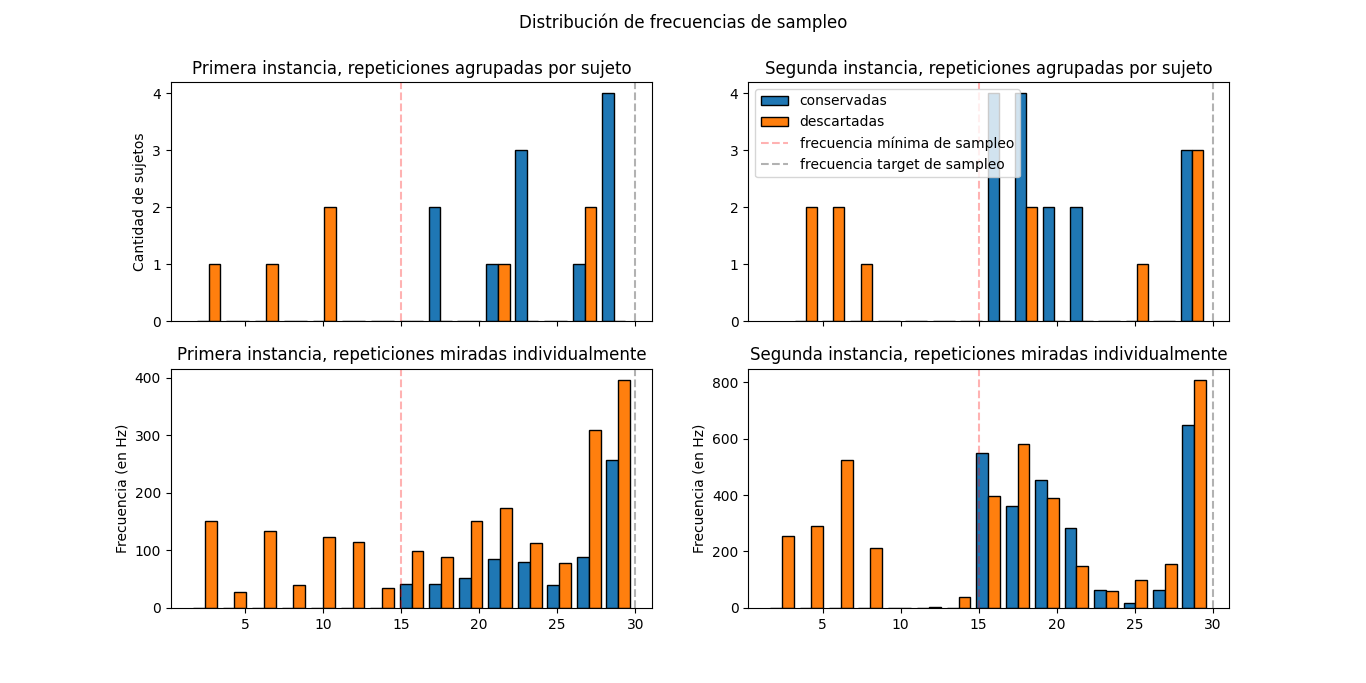
\includegraphics[width=\textwidth]{metodo/sampling-frequency-distribution.png}
  \caption{Distribución de frecuencias de muestreo}
  [TODO: Regenerar plot y ajustar dimensiones]
  \label{fig:sampling-frequency-distribution}
\end{figure}

\begin{figure}
  \centering
  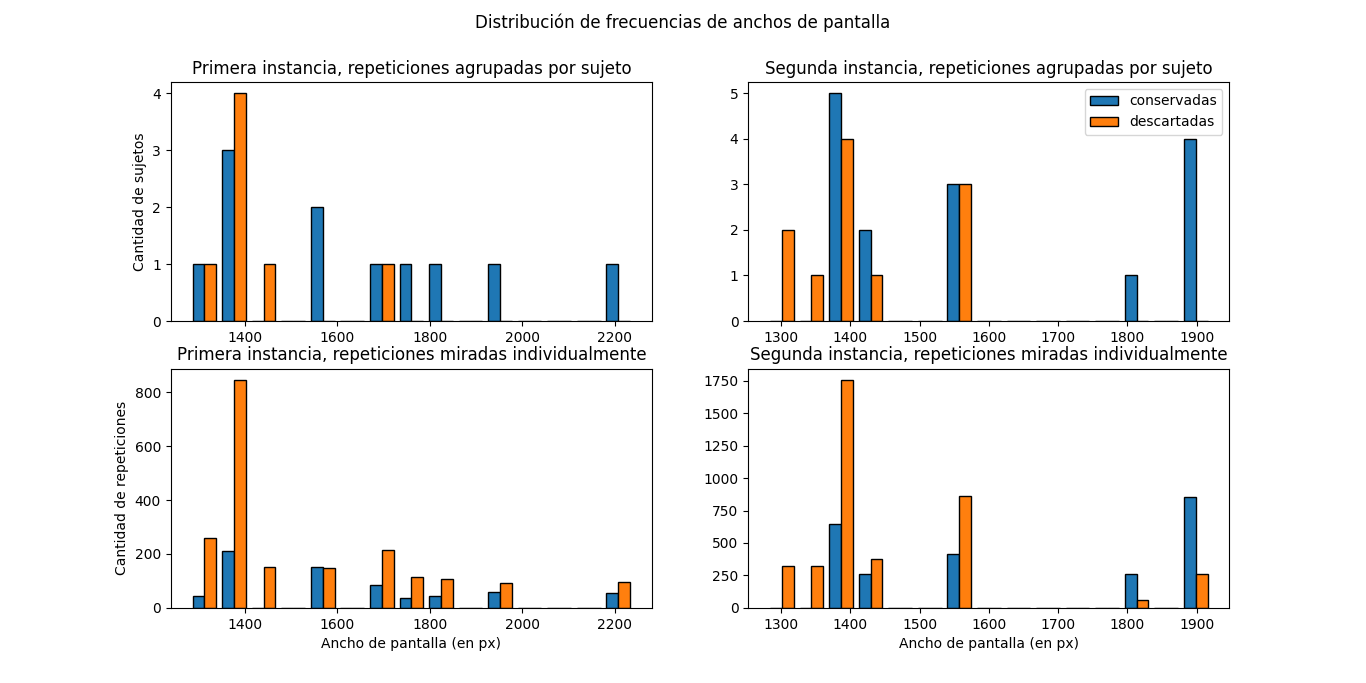
\includegraphics[width=\textwidth]{metodo/widths-distribution.png}
  \caption{Distribución de anchos de resoluciones}
  [TODO: Regenerar plot y ajustar dimensiones]
  \label{fig:widths-distribution}
\end{figure}

En primer lugar, se descartaron las repeticiones cuyas estimaciones tuvieran
una frecuencia menor a 15 Hz.
Luego, a frecuencia de muestreo se uniformizó a 30 Hz realizando interpolación
lineal.
A partir del timestamp de la primera muestra se tomaron timestamps subsecuentes
cada 1000 / 30 ms.
Para cada uno de estos timestamps se interpoló la estimación correspondiente
utilizando la estimación anterior y la estimación posterior. 

[TODO: Retrabajar la explicación de las normalización y capaz agregar un diagrama]

Las estimaciones de la mirada fueron luego llevadas del rango variable por
sujeto al rango [-1, 1] buscando que al valor 0 fueran a caer las estimaciones
correspondientes a cuando el sujeto miraba al centro de la pantalla.
En la primera, instancia se normalizó cada tarea individualmente utilizando el
centro estimado de cada sujeto c (calculado como el promedio de los valores de
tal sujeto) y los valores mínimos $min_x$ y máximos $max_x$ de la repetición:
las estimaciones en el rango [$min_x$, c] se llevaron con interpolación lineal
al rango [-1, 0] y análogamente las estimaciones en el rango [c, $max_x$] se
llevaron al rango [0, 1].
Para la segunda instancia, la normalización se realizó en base a las
validaciones realizadas durante la tarea.
Para cada conjunto de repeticiones posteriores a una calibración + validación
se calcularon los valores l, c y r como el promedio de las estimaciones
obtenidas al mostrar respectivamente los estímulos de validación a izquierda,
centro y derecha.
Luego, similar a la instancia anterior, el rango [l, c] fue llevado al rango
[-1, 0] y el rango [c, r] fue llevado al rango [0, 1].

Post normalización, las estimaciones fueron modificadas tal que pudiera
asumirse que el estímulo lateral aparecía siempre del mismo lado.
Para esto, en las repeticiones en las cuales el estímulo visual aparecía a la
izquierda, se multiplicaron los valores de las estimaciones horizontales por
-1.
De esta manera se podrá asumir que si los valores de las estimaciones son
positivos entonces el sujeto miró al estímulo, mientras que si las estimaciones
son negativas entonces el sujeto habrá mirado en la dirección contraria.
Así, para identificar prosacadas correctas tendrá que verificarse que haya un
salto de valores cercanos a 0 a valores cercanos a 1, y análogamente para
identificar antisacadas correctas tendrá que verificarse un salto de valores
cercanos a 0 a valores cercanos a -1.

Se descartaron luego las repeticiones en las cuales el sujeto no estuviera
fijando la posición del estímulo de fijación durante los 500 ms previos a la
aparición del estímulo visual lateral.
Si un sujeto terminó con menos de 30 de repeticiones por tarea entonces se
descartó también el resto de sus repeticiones.
Además se descartaron a mano las repeticiones de sujetos cuyos datos se
considerarán inválidos.


\documentclass[aspectratio=169]{beamer}

\usepackage{subcaption}
\usepackage{emoji}

\title{Evaluación y desarrollo de \textit{eye tracking} remoto en navegadores
\textit{web}}
\author{Francisco Figari, Juan Kamienkowski, Gustavo Juantorena, Bruno Bianchi}
\date{Buenos Aires, 2022}
\titlegraphic{
\includegraphics[width=8em]{img/logo-fcen.png}}

\setbeamertemplate{navigation symbols}{}

% TODO: Hacer que esto sea opcional
\setbeamertemplate{frametitle}{
  \insertsectionhead\par
  \vspace*{0.2mm}
  \insertsubsectionhead\par
  \vspace*{0.2mm}
  \insertframetitle
}

\begin{document}

\frame{\titlepage}

\section{Implementación}

\begin{frame}{\texttt{WebGazer} como punto de partida}

  \begin{columns}
    \begin{column}{.5\textwidth}
      \begin{itemize}
        \item[\emoji{thumbs-up}] Extracción de frames a través de la API del
          navegador
        \item[\emoji{thumbs-up}] Modelos de localización de los ojos y de
          estimación de la mirada
        \item[\emoji{thumbs-down}] Calibración inadecuada
        \item[\emoji{thumbs-down}] Ausencia de notificación de descalibraciones
        \item[\emoji{party-popper}] Corrregida falla de \texttt{WebGazer} que
          causaba \textit{crashes} del navegador en ciertas notebooks
      \end{itemize}
    \end{column}

    \begin{column}{.5\textwidth}
      \begin{figure}
        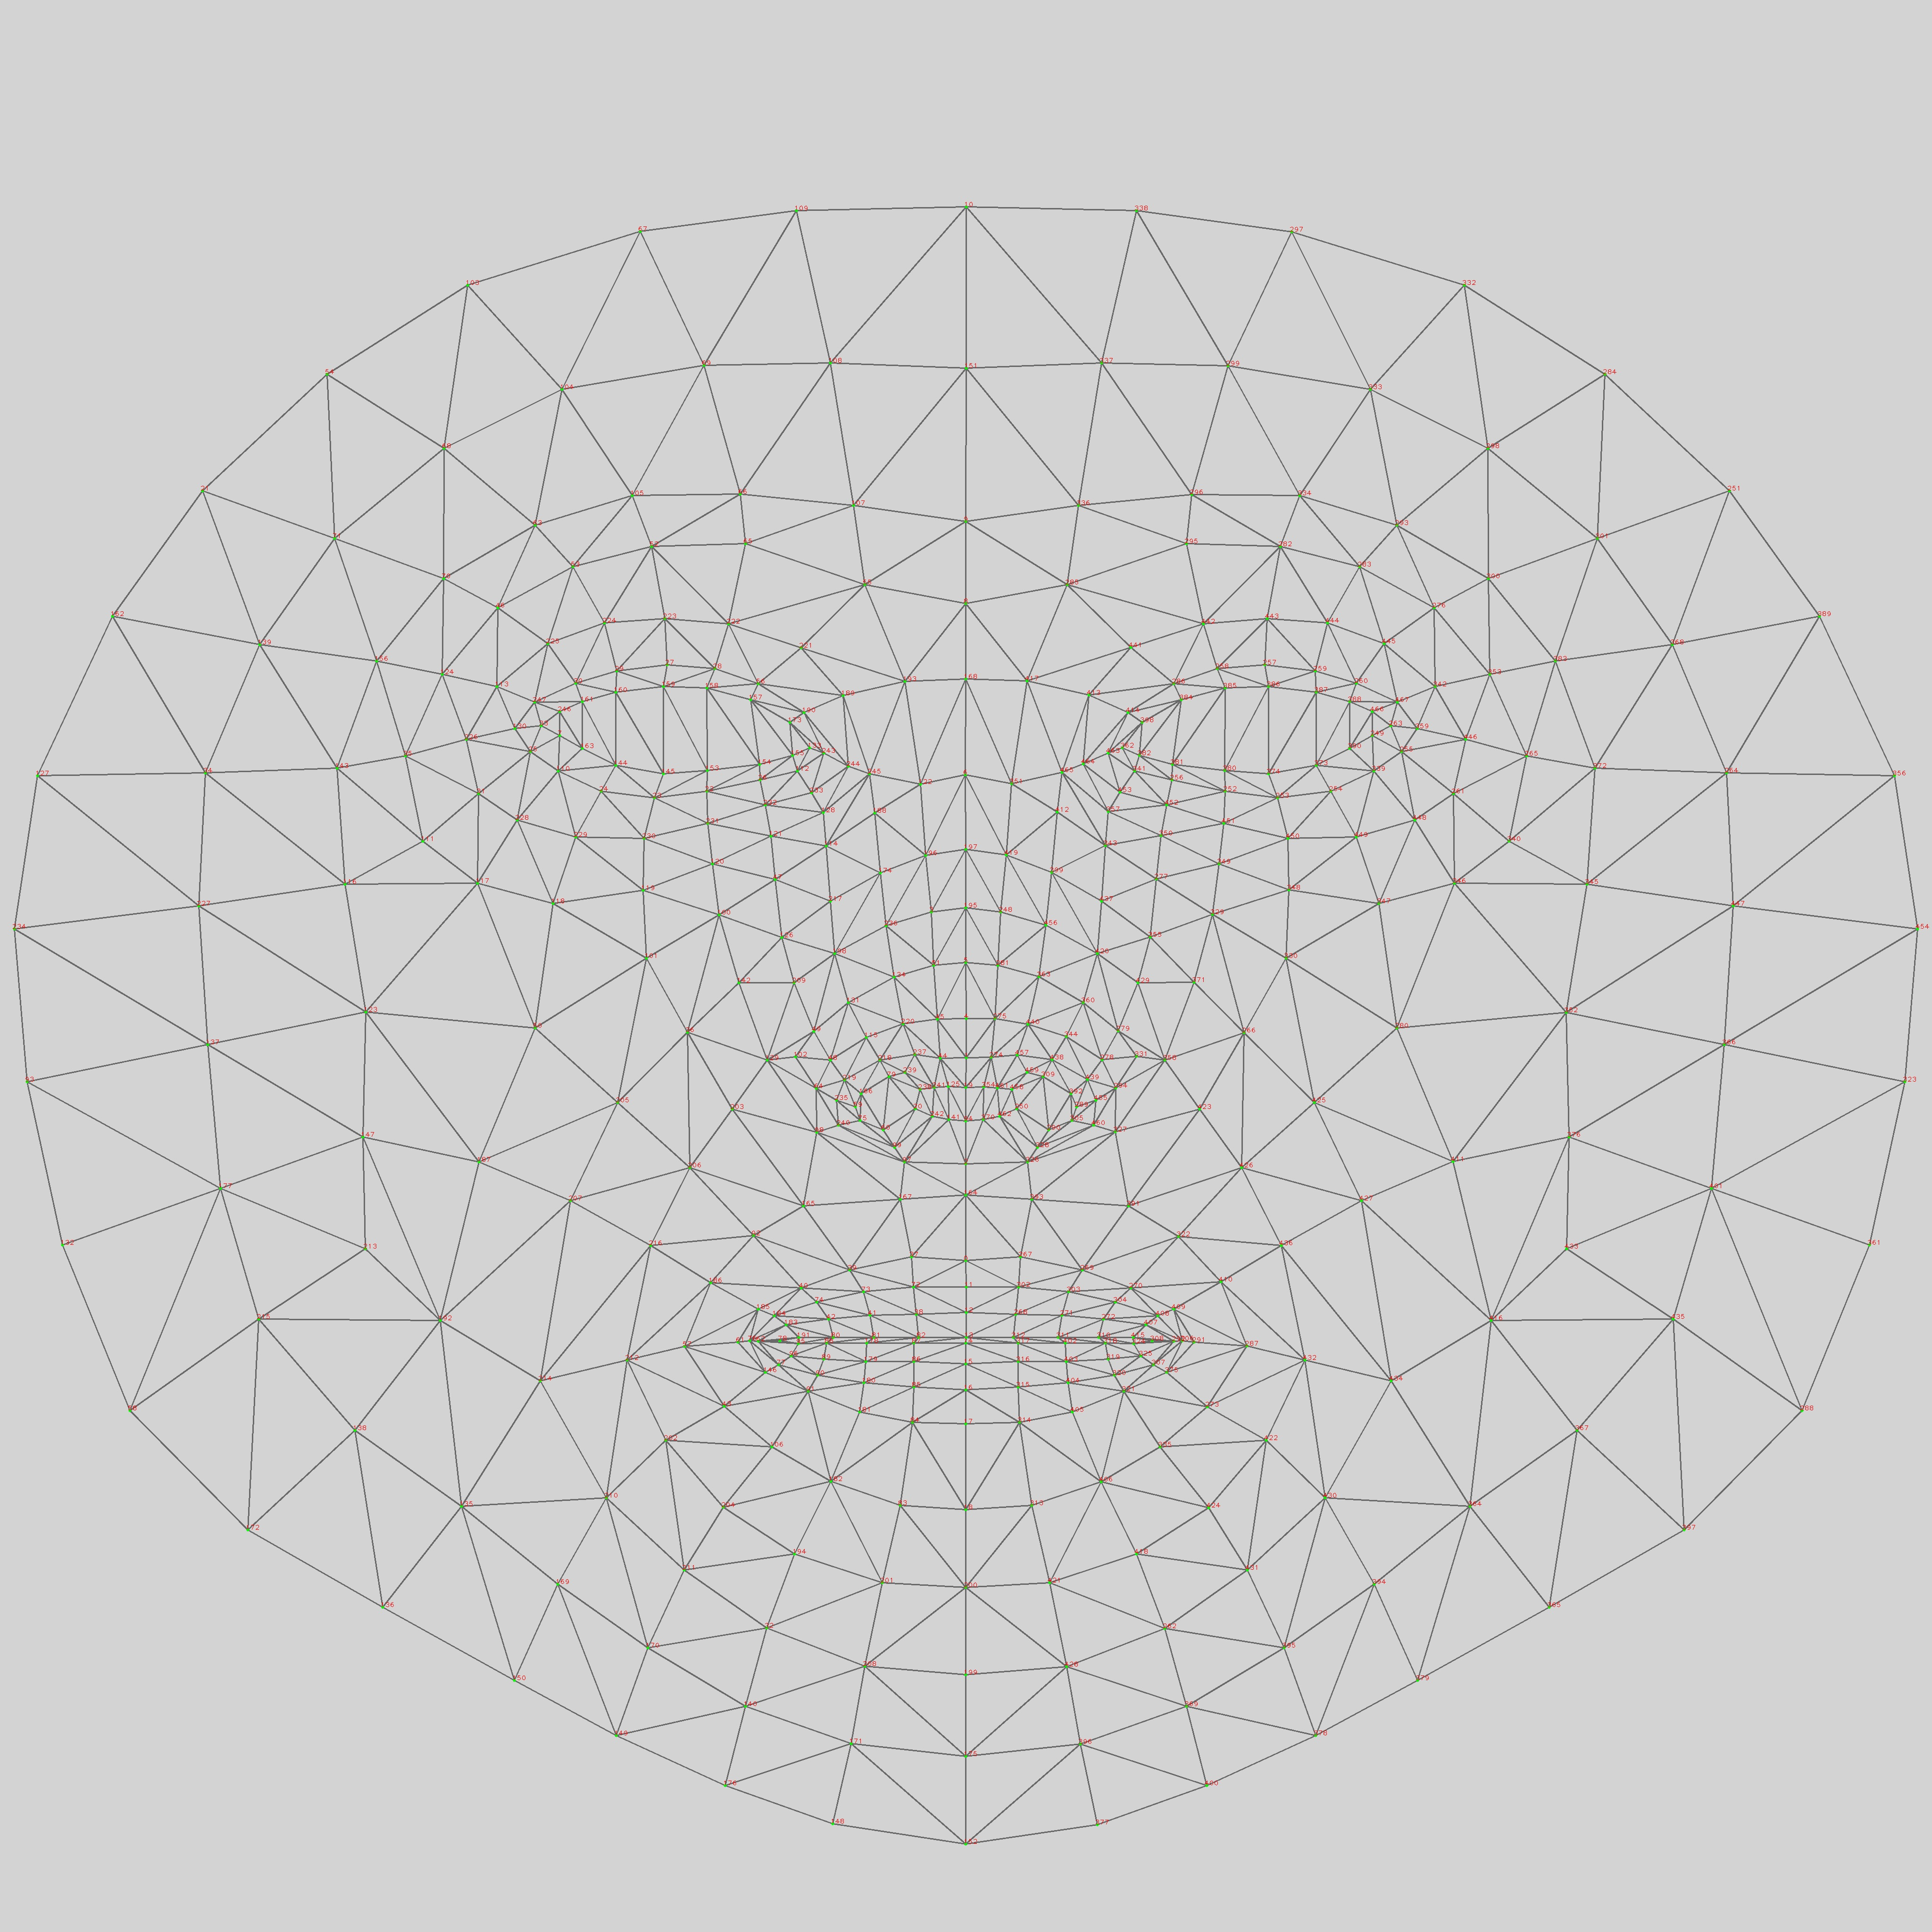
\includegraphics[width=0.75\linewidth]{img/facemesh-kepyoints.jpg}
        \caption{\textit{Output} del modelo de \textit{facemesh} utilizado por
        \texttt{WebGazer} para la localización de los ojos}
      \end{figure}
    \end{column}
  \end{columns}

\end{frame}

\begin{frame}{Calibración y validación}
  \begin{itemize}
    \item Nuestro caso de uso no garantiza interacciones

    \item Se muestran una serie de puntos, para cada uno de los cuales el
      usuario tendrá que fijar la mirada y presionar la barra de espacio
    
    \item Validación post calibración implementada de similar manera

    \item[\emoji{party-popper}] \texttt{WebGazer} adaptado para evitar cómputos
      ya no necesarios
  \end{itemize}
\end{frame}

\begin{frame}{Notificación de descalibración}

  \begin{columns}
    \begin{column}{.5\textwidth}
      \begin{itemize}
        \item Basada en detectar movimiento
        \item Instanciada luego de cada calibración
        \item Verificación realizada para cada \textit{frame}
        \item \emoji{party-popper} \texttt{WebGazer} adaptado para exponer los
          recuadros calculados en cada \textit{frame} por la rutina de
          localización de ojos
      \end{itemize}
    \end{column}

    \begin{column}{.5\textwidth}
      \begin{figure}
        \centering
        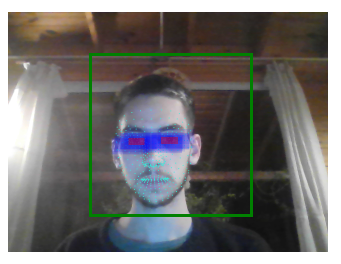
\includegraphics[width=\textwidth]{img/eyetracker-playground-screenshot.png}
        \caption{Detección de movimiento en funcionamiento}
      \end{figure}
    \end{column}
  \end{columns}

\end{frame}

\section{Experimentación}

\begin{frame}{Caso de estudio: tarea de antisacadas}

  \begin{columns}
    \begin{column}{.5\textwidth}
      \begin{itemize}
        \item Clínicamente relevante
        \item Resultados esperados ya establecidos
        \item Tarea simple para validar movimientos oculares
      \end{itemize}
    \end{column}
    \begin{column}{.5\textwidth}
      \begin{figure}
        \centering
        \includegraphics[width=\linewidth]{img/antisaccades-protocol.png}
        \caption{Protocolo de las tareas}
      \end{figure}
    \end{column}
  \end{columns}

\end{frame}

\begin{frame}{Primera instancia}
  \begin{itemize}
    \item Limitados a 10 minutos debido a una falla de \texttt{WebGazer}
    \item Únicamente ensayos de antisacada
    \item Recalibración luego de cada notificación de descalibración
    \item Sin validación post calibración
  \end{itemize}
\end{frame}

\begin{frame}{Segunda instancia}
  \begin{itemize}
    \item Duración superior a 20 minutos
    \item Ensayos de prosacadas y de antisacadas
    \item Recalibración cada 10 ensayos y sólo si se detectó una
      descalibración
    \item Con validación post calibración
  \end{itemize}
\end{frame}

\begin{frame}{Implementación y distribución}

  \begin{columns}
    \begin{column}{0.4\textwidth}
      \begin{figure}
        \centering
        
\includegraphics[width=\textwidth]{img/jspsych-logo.jpg}
      \end{figure}
    \end{column}
    \begin{column}{0.6\textwidth}
      \begin{figure}
        \centering
        
\includegraphics[width=0.8\textwidth]{img/cognition-run-logo.png}
        
\includegraphics[width=\textwidth]{img/neuropruebas-logo.jpg}
      \end{figure}
    \end{column}
  \end{columns}
\end{frame}


\section{Resultados}

\begin{frame}{Ejemplo de \textit{output} del sistema}
  \begin{figure}
    \centering
    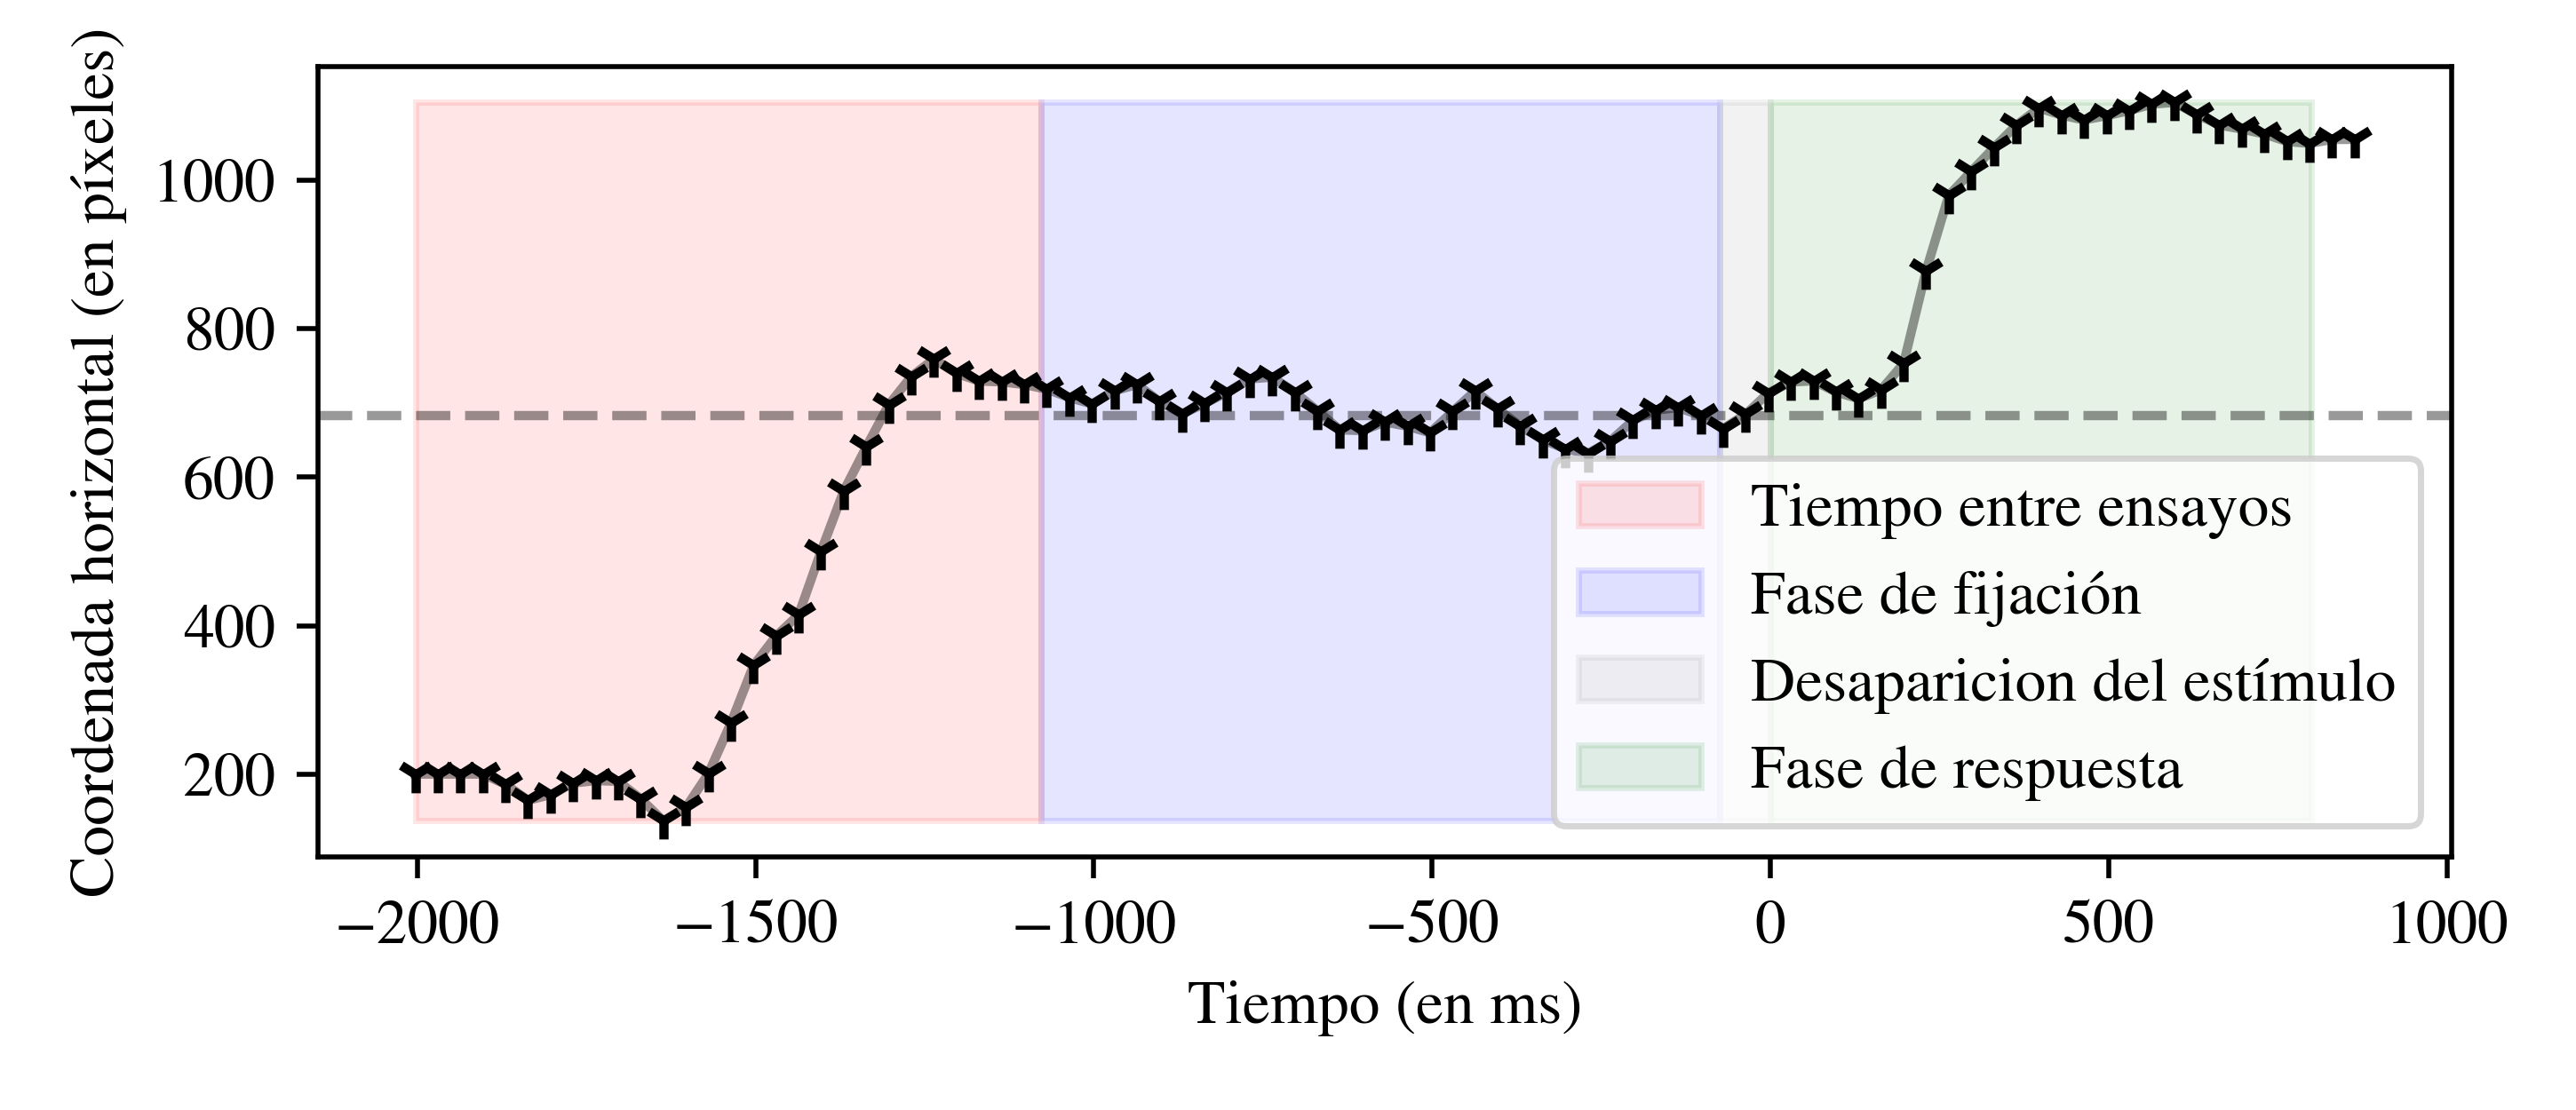
\includegraphics[width=\linewidth]{plots/output-example.png}
  \end{figure}
\end{frame}

\begin{frame}{Frecuencias de muestreo}
  \begin{figure}
    \centering
    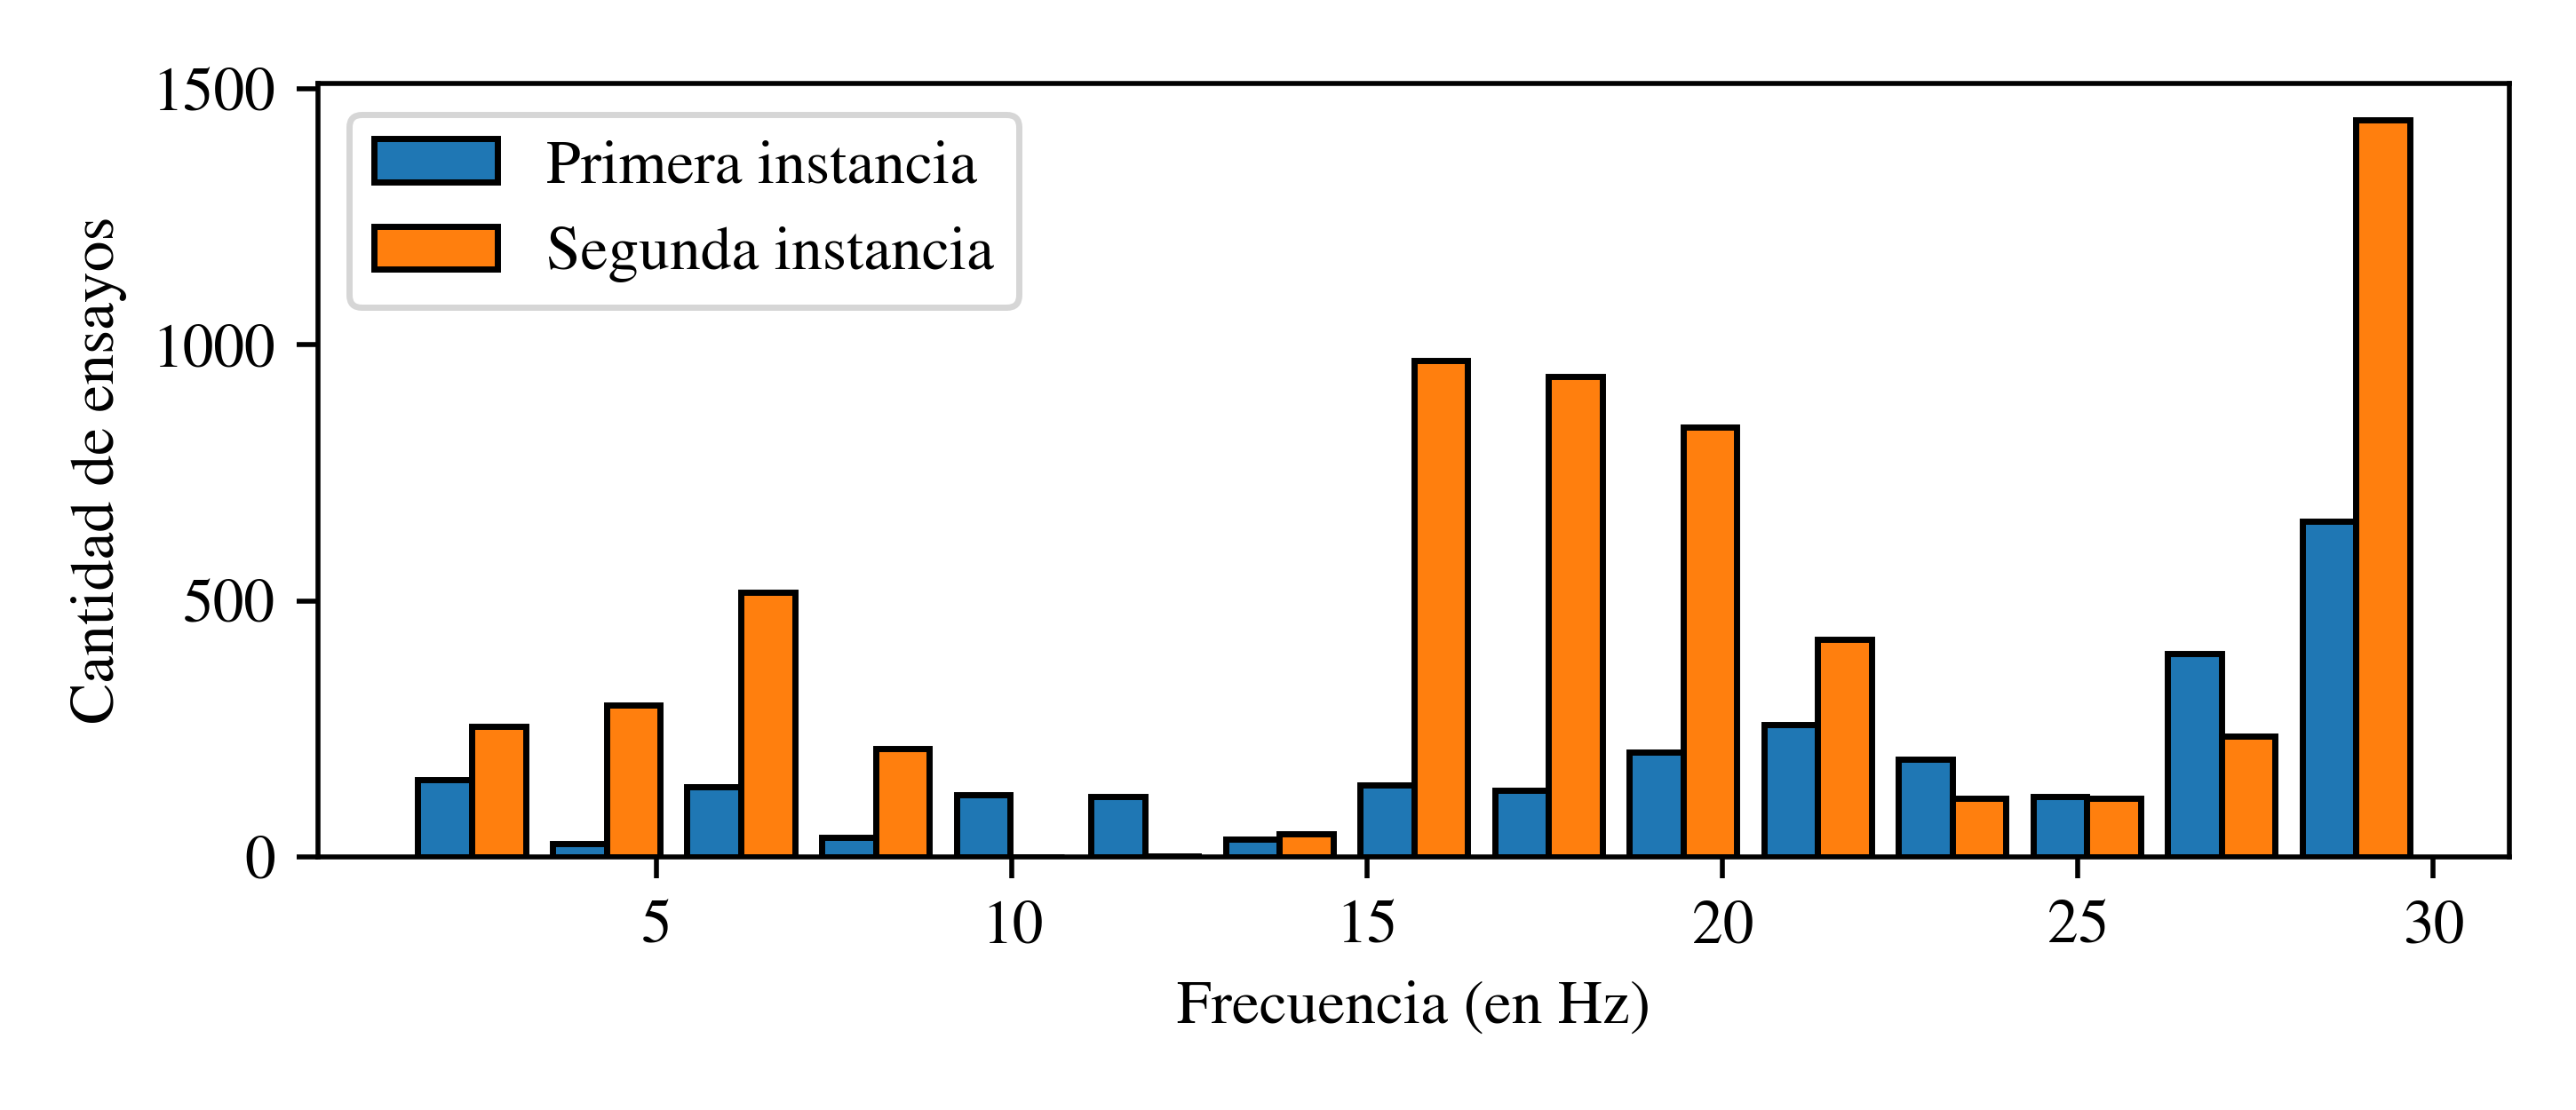
\includegraphics[width=\linewidth]{plots/sampling-frequencies-distribution.png}
  \end{figure}
\end{frame}

\begin{frame}{Anchos de pantalla}
  \begin{figure}
    \centering
    \includegraphics[width=\linewidth]{plots/screens-widths-distribution.png}
  \end{figure}
\end{frame}

\begin{frame}{Estimaciones desviadas}
  \begin{figure}
    \centering
    \includegraphics[width=\linewidth]{plots/skewed-estimations-examples.png}
    \caption{Las estimaciones de algunos sujetos están desviadas de los valores reales}
  \end{figure}
\end{frame}

\begin{frame}{Limpieza y normalización}
  \begin{columns}
    \begin{column}{0.4\textwidth}
      \begin{itemize}
        \item Ensayos descartados: \begin{itemize}
          \item frecuencia menor a 15 Hz
          \item a mano
          \item si el sujeto se distrajo de la tarea
        \end{itemize}
        \item Frecuencia de muestreo: \textit{Upsampling} a 30 Hz usando
          interpolación lineal
      \end{itemize}
    \end{column}
    \begin{column}{0.6\textwidth}
      \begin{figure}
        \centering
        \includegraphics[width=\linewidth]{plots/normalization-example.png}
        \caption{Normalizado y espejado}
      \end{figure}
    \end{column}
  \end{columns}
\end{frame}

\begin{frame}{Detección de sacadas}
  \begin{columns}
    \begin{column}{0.5\textwidth}
      \begin{figure}
        \centering
        \includegraphics[width=\linewidth]{img/saccades-example.jpg}
        \caption{Los movimientos oculares muestran qué elementos de una imagen
        capturan la atención}
      \end{figure}
    \end{column}
    \begin{column}{0.5\textwidth}
      \begin{figure}
        \centering
        \includegraphics[width=\linewidth]{plots/detected-saccades-example.png}
        \caption{Sacadas detectadas sobre las estimaciones de un ensayo}
      \end{figure}
    \end{column}
  \end{columns}
\end{frame}

\begin{frame}{Conclusiones generales replicadas}
  \begin{table}
    \centering
    \begin{tabular}{ l | c | c | c }
      & correctitud & \multicolumn{2}{ c }{tiempo de respuesta (ms)} \\
      &             & correcto & incorrecto \\
      \hline
      antisacada & 81.29\% & 509 (93) & 346 (105) \\
    \end{tabular}
    \caption{Primera instancia}
  \end{table}
  
  \begin{table}
    \centering
    \begin{tabular}{ l | c | c | c }
      & correctitud & \multicolumn{2}{ c }{tiempo de respuesta (ms)} \\
      &             & correcto & incorrecto \\
      \hline
      antisacada & 94.82\% & 358 (109) & 299 (103) \\
      \hline
      prosacada & 98.09\% & 320 (108) & 311 (150) \\
    \end{tabular}
    \caption{Segunda instancia}
  \end{table}

  % TODO: Poner marker negativo acá
  En la bibliografía para la tarea de antisacadas se reportan \textbf{valores
  de correctitud} más cercanos al rango $[60\%, 75\%]$.
\end{frame}

\begin{frame}{Menos datos de lo esperado}
  \begin{columns}
    \begin{column}{0.4\textwidth}
      \begin{itemize}
        \item Cantidad de ensayos iniciales baja en relación a otros trabajos
        \item Descarte de aproximadamente $\frac{2}{3}$ de los datos
        \item Altas e inesperadas tasas de correctitud
      \end{itemize}
    \end{column}

    \begin{column}{0.6\textwidth}
      \begin{table}
        \centering

        \begin{tabular}{ l | c | c }
          Antisacadas   & incorrecto  & correcto \\
          \hline
          \# total      & 64          & 1173 \\
          \hline
          \# por sujeto & 4.57 (2.84) & 78.20 (40.38)
        \end{tabular}

        \vspace{0.3cm}

        \begin{tabular}{ l | c | c }
          Prosacadas    & incorrecto  & correcto \\
          \hline
          \# total      & 22          & 1134 \\
          \hline
          \# por sujeto & 2.44 (1.23) & 75.59 (38.58)
        \end{tabular}

        \caption{Desbalance entre grupos incorrecto y grupo correcto}
      \end{table}
    \end{column}
  \end{columns}
\end{frame}

\begin{frame}{~}
  fin
\end{frame}

\section{Motivación}

\begin{frame}{~}

  \begin{itemize}
      \item Los ojos como entrada a los procesos cognitivos y estados
        emocionales de una persona
      \item Frecuentemente estudiados en el contexto de la neuropsicología
        digital para estimar el comportamiento
      \item Importante incluso cuando no son el foco del análisis
        (\textit{e.g.}, detección de caras)
      % utilizado también en el desarollo HMI, en el estudio de usabilidad de
      % interfaces, recientemente en el campo de la oftalmología para estimar
      % el campo visual
      \item Usos en otras disciplinas
  \end{itemize}

  \begin{figure}
    \begin{subfigure}{0.49\textwidth}
      \centering
      \includegraphics[width=\linewidth]{img/eye-link-eeg.jpg}
      \caption{\textit{Eye tracking} combinado con electroencefalograma}
    \end{subfigure}
    \begin{subfigure}{0.49\textwidth}
      \centering
      \includegraphics[width=\linewidth]{img/reading-fixations-saccades.jpg}
      \caption{Estimación de la mirada durante una tarea de lectura}
    \end{subfigure}
  \end{figure}

\end{frame}

\begin{frame}{~}

  \begin{itemize}
    \item Comunmente resuelto con sistemas comerciales cerrados
    \item Costos altos (entre 5000 y 40000 euros) mientras que el hardware en
      sí representa una pequeña fracción de estos (entre 200 y 600 euros)

    % si falta algún dato (e.g., la precisión del diámetro de la pupila) no
    % se lo puede saber
    \item Imposibilidad de auditar la implementación
    \item Necesidad de asistir a un laboratorio
  \end{itemize}

  \begin{figure}
    \begin{subfigure}{0.49\textwidth}
      \centering
      \includegraphics[width=0.6\linewidth]{img/eye-link-chinrest.jpg}
      \caption{La reestricción de movimiento facilita mantener calibrado el
      sistema}
    \end{subfigure}
    \begin{subfigure}{0.49\textwidth}
      \centering
      \includegraphics[width=0.5\linewidth]{img/eye-tracker-head-mounted.jpg}
      \caption{\textit{Eye tracker} montado a la cabeza}
    \end{subfigure}
  \end{figure}

\end{frame}

\begin{frame}{~}

  \begin{columns}
    \begin{column}{0.4\textwidth}
      \begin{itemize}
        \item Interés en proveer software de \textit{eye tracking}

        \item Posibilidad de \textit{crowdsourcing}

          % e.g., detectar pérdidas de atención en clases masivas
        \item Potencial para nuevas aplicaciones
      \end{itemize}

    \end{column}
    \begin{column}{0.6\textwidth}

      \begin{figure}
        \begin{subfigure}{0.49\textwidth}
          \centering
          \includegraphics[width=0.8\linewidth]{img/external-webcam.jpg}
        \end{subfigure}
        \begin{subfigure}{0.49\textwidth}
          \centering
          \includegraphics[width=0.8\linewidth]{img/notebook.jpg}
        \end{subfigure}
        \caption{Webcams domésticas ya disponibles}
      \end{figure}

      \begin{figure}
        \begin{subfigure}{0.49\textwidth}
          \centering
          \includegraphics[width=0.6\linewidth]{img/basler-camera.jpg}
        \end{subfigure}
        \begin{subfigure}{0.49\textwidth}
          \centering
          \includegraphics[width=0.8\linewidth]{img/basler-cameras-with-lens.png}
        \end{subfigure}
        \caption{Hardware profesional adquirible por una fracción del costo}
      \end{figure}


    \end{column}
  \end{columns}
\end{frame}

\section{Objetivos}

\begin{frame}{~}

  \begin{itemize}
    \item Evaluar implementaciones recientes con similares motivaciones
    % - entender el problema
    % - definir los requerimientos
    % - establecer qué puede reutilizarse

    \item Implementar un prototipo de \textit{eye tracker} que corra en
      navegadores \textit{web} y que esté orientado a análisis clínicos
    % - adaptar lo que pudiera reutilizarse
    % - implementar los módulos que faltaran

    \item Emular análisis clínicos remotos y recolectar datos utilizando el
      prototipo implementado

    \item Establecer la capacidad del prototipo en replicar conclusiones
      establecidas con \textit{eye trackers} profesionales de laboratorio

  \end{itemize}

\end{frame}

\section{Desarmando el problema de \textit{eye tracking} web}

\begin{frame}{~}
  \begin{columns}
    \begin{column}{0.5\textwidth}
      \begin{itemize}
        \item Estimar qué coordenada de la pantalla está mirando el usuario en
          un contexto de estudios clínicos
        \item Un \textit{stream} de frames de la webcam como \textit{input}
        \item Se divide en \textbf{localizar los ojos} y luego \textbf{estimar
          la mirada}
        \item Calibraciones necesarias en cada sesión de uso
      \end{itemize}
    \end{column}
    \begin{column}{0.5\textwidth}
      \begin{figure}
        \centering
        TODO: Reemplazar esto por un único plot que ejemplifique el output
        deseado
        \includegraphics[width=\linewidth]{img/eye-tracking-output-example.png}
        \caption{Sacadas detectadas sobre serie de tiempo de la coordenada x}
      \end{figure}
    \end{column}
  \end{columns}
\end{frame}

\begin{frame}{~}
    \begin{itemize}
    \item Resultados consistentes dentro de una misma población
    % - mayor tasa de correctitud para los casos de prosacada que para aquellos de antisacada
    % - para los grupos correctos se esperan mayores tiempos de respuesta en las repeticiones de antisacadas que en aquellas de prosacadas
    % - a mayor edad menor rendimiento en la tarea, tanto en latencia como en correctitud

    \item Búsqueda de establecer resultados para poblaciones de distinta condición neuropsicológica
    % - ditintos tipos de lesiones cerebrales
    % - déficit de atención, esquizofrenia, síndrome de Parkinson, síndrome de Tourette
    % - individuos sanos, efectos de la edad

    \item Comparación dificultosa entre distintos trabajos
    % - se obtienen valores del mismo orden (RT y correctitud) para pacientes sanos en un estudio que para pacientes con esquizofrenia de otro estudio
    \end{itemize}

\end{frame}

\section{Alternativas al \textit{eye tracking} tradicional}

\subsection{Trabajos previos}

\begin{frame}{~}

  TODO: Separar esto en varios frames
  \begin{itemize}
    \item \texttt{PupilEXT}: software para realizar pupilometría; deben
      proveerse cámaras profesionales y emisores de luz infrarroja; TODO:
      imagen pupilometría

    % hay que resaltar la importancia de esto de analizar el momento de mayor
    % coincidencia
    \item \texttt{PACE}: aplicación de escritorio basada en webcam; calibran en
      base a interacciones del usuario; analizar el momento de mayor
      coincidencia entre la mirada y la posición de la interacción; TODO:
      alguna imagen del paper

    \item \texttt{TurkerGaze}: aplicación web basada en webcam; generación de
      mapas de saliencia a través de \textit{crowdsourcing}; TODO: imagen mapas
      de saliencia

    \item \texttt{WebGazer}: aplicación web basada en webcam; se basan en
      \texttt{PACE} y \texttt{TurkerGaze}; provisto en forma de paquete; TODO:
      screenshot del paquete

  \end{itemize}

\end{frame}

\subsection{Implicancias del contexto remoto de navegador \textit{web}}

\begin{frame}{~}

  \begin{itemize}
    \item[+] Posibilidad de reutilizar cámaras web

    \item[+] Compatibilidad con otras herramientas web, en particular
      \texttt{JSPsych}

    % no es el fin del mundo pero es un lenguaje bastante odiado e implica
    % dificultades en cuanto a la precisión. Por ejemplo, la duración de cada
    % frame va a ser variable, lo que dificulta mostrar estímulos durante
    % cortas cantidades de tiempo
    \item Necesidad de implementar sobre JavaScript

    % no sólo las webcams son variables si no que tmb la compu donde corre el 
    % programa
    \item[--] Hardware variable de potencialmente bajo rendimiento

    % deben transmitirse en texto e imagenes sin que puedan hacerse
    % aclaraciones en el momento. esto implica una duración total del
    % experimento potencialmente mayor
    \item[--] Las instrucciones no pueden ser transmitidas en persona

    % puede variar la luz o la disposición del hardware
    \item[--] Ambiente físico no controlado
  \end{itemize}

  TODO: Screenshots de JSPsych y de Amazon Mechanical Turk

\end{frame}

\subsection{Modelado de la mirada}

\begin{frame}{~}
  \begin{itemize}
    % no entrar en detalle con esto pero mencionar brevemente por qué
    \item Limitados a una pequeña fracción de la bibliografía debido a tener
      una y sólo una cámara
    
    % acuerdo en que hay que mostar una serie de puntos pero no está claro
    % cuántos, ni cómo, ni qué información rescatar. tmb hay interés en
    % minimizar la duración del exp
    \item Falta de estándar respecto de cómo calibrar

    % ante ligeros movimientos de cabeza el sistema va a quedar descalibrado.
    % hay que tenerlo en cuenta en el flow del experimento. puede recalibrarse
    % cada un tiempo fijo (TG), agregar data de calibración a medida que avanza
    % el experimento (WG) o bien implementarse alguna heurística para decidir
    % cuándo el sistema necesita una recalibración
    \item Ausencia de invarianza frente a movimientos de cabeza y de
      reestricción de movimiento
  \end{itemize}
\end{frame}

\section{Implementación}

\section{Experimentación}

\section{Resultados}

\subsection{Características de los datos}

\begin{frame}{Frecuencias de muestreo}

  TODO: Acomodar subplots y mostrarlo solo por estimaciones para que sea menos
  lío
  \begin{figure}
    \includegraphics[width=0.7\linewidth]{img/second-sampling-frequencies-distribution.png}
  \end{figure}

\end{frame}

\begin{frame}{Anchos de pantalla}

  TODO: Acomodar subplots y mostrarlo solo por estimaciones para que sea menos
  lío
  \begin{figure}
    \includegraphics[width=0.7\linewidth]{img/second-widths-distribution.png}
  \end{figure}

\end{frame}

\begin{frame}{Estimaciones desviadas}

  TODO: Acomodar subplots
  \begin{figure}
    \includegraphics[width=0.8\linewidth]{img/skewed-estimations-examples.png}
  \end{figure}

\end{frame}

\subsection{Limpieza y normalización}

\subsection{Detección de sacadas}

\begin{frame}{~}

  Luego de normalizar, se considerará un intervalo como una sacada si:
  \begin{enumerate}
    \item La mirada se mueve en una misma dirección
    \item El intervalo dura al menos 40 ms
    \item Se recorre \textit{cierta} distancia mínima durante ese intervalo
    \item El desplazamiento es lo \textit{suficientemente rápido}
  \end{enumerate}
  Implementación \textit{ad hoc} cuya calidad no fue estudiada.

\end{frame}

\subsection{Conclusiones generales replicadas}

\begin{frame}{~}
  \begin{columns}
    \begin{column}{0.5\textwidth}
      \begin{figure}
        \centering
        \includegraphics[width=\linewidth]{img/second-disaggregated-prosaccades.png}
      \end{figure}
    \end{column}
    \begin{column}{0.5\textwidth}
      \begin{figure}
        \centering
        \includegraphics[width=\linewidth]{img/second-disaggregated-antisaccades.png}
      \end{figure}
    \end{column}
  \end{columns}
\end{frame}

\subsection{Grupos etarios no representados}

\begin{frame}{~}
  TODO: Cambiarlo para que sólo muestre los sujetos y no los ensayos
  \begin{columns}
    \begin{column}{0.5\textwidth}
  \begin{figure}
    \centering
    \includegraphics[width=\linewidth]{img/first-ages-distribution.png}
    \caption{Primera instancia}
  \end{figure}
      
    \end{column}
    \begin{column}{0.5\textwidth}
  \begin{figure}
    \centering
    \includegraphics[width=\linewidth]{img/second-ages-distribution.png}
    \caption{Segunda instancia}
  \end{figure}
    \end{column}
  \end{columns}
\end{frame}

\subsection{Menos datos de lo esperado}



\section{Conclusiones}

\begin{frame}{~}
  \begin{itemize}
    \item Se obtuvo un prototipo de \textit{eye tracker} para navegadores web
    \item Potencial para realizar análisis clínicos remotos
    \item Campo aún en sus primeros pasos
    \item Precisión muy por debajo de aquella alcanzable por \textit{eye
      trackers} profesionales
  \end{itemize}
\end{frame}

\subsection{Limitaciones}

\begin{frame}{Implementativas}
  TODO: Las limitaciones y trabajo futuro no ponerlas todas y en cambio referir
  a la tesis \par

. bajas frecuencias
. pestañeos
. estimación del tamaño de la pantalla
. imprecisión en la duración de cada frame, problemático si se quiere mostrar
  un estímulo durante una corta duración de tiempo

  \begin{figure}
    \centering
    \includegraphics[width=0.9\linewidth]{img/undetected-saccades-examples.png}
    \caption{Ejemplos de sacadas no detectadas}
  \end{figure}
\end{frame}

\begin{frame}{Experimentales}
. proporción de datos filtrados demasiado elevada
. necesidad de revisar la causa de las altas tasas de correctitud obtenidas
. representatividad de distintos grupos etarios
\end{frame}

\subsection{Trabajo futuro}

\begin{frame}{Análisis de datos}
. Investigar e implementar mecanismos estándares de detección de sacadas, lo
  cual podría basarse en la previa construcción de un dataset etiquetado de
  sacadas
. Revisar criterios de exclusión para asegurarse de no estar filtrando datos
  válidos
. Realizar nuevas rondas de experimentación, estimando previamente la cantidad
  de ensayos necesarios para asegurar cantidades suficientes en los grupos
  incorrectos y en los distintos grupos etarios
\end{frame}

\begin{frame}{Análisis de sensibilidad}
. propuesta sobre experimento para recolectar datos y establecer métricas de
  calidad sobre las estimaciones obtenidas por la herramienta
TODO: Acá combinar un poco lo que quedó en la tesis y lo que pensé para
      sensitivity analysis
\end{frame}

\begin{frame}{Prototipo desarrollado}
. optimizar frecuencia de muestreo
. reexplorar detección de descalibraciones y qué significa que el sistema esté
  descalibrado
. mejorar la calibración, generalizarla a más puntos de interés
. detección de pestañeos
. estimación del tamaño de la pantalla y posibilidad de mostrar estímulos en
  grados
. verificación de condiciones iniciales
TODO: Extender con lo que haya escrito en la tesis
\end{frame}

\begin{frame}{\textit{Eye tracking} en navegadores \textit{web}}
. extender bibliografía que aplique a nuestro contexto
. eye tracking web no podría atacar algunos problemas que sí puede el eye
  tracking tradicional, pero al ser remoto y de bajo costo es posible que
  permita atacar nuevos problemas. Deben entonces buscarse tales problemas
\end{frame}

\end{document}


\chapter{Conclusiones}

\printbibliography
\backmatter

\end{document}
